%%%%%%%% ICML 2023 EXAMPLE LATEX SUBMISSION FILE %%%%%%%%%%%%%%%%%

\documentclass{article}

% Recommended, but optional, packages for figures and better typesetting:
\usepackage{microtype}
\usepackage{graphicx}
\usepackage{subfigure}
\usepackage{caption}
\usepackage{subcaption}
\usepackage{booktabs} % for professional tables

% hyperref makes hyperlinks in the resulting PDF.
% If your build breaks (sometimes temporarily if a hyperlink spans a page)
% please comment out the following usepackage line and replace
% \usepackage{icml2023} with \usepackage[nohyperref]{icml2023} above.
\usepackage{hyperref}

% Attempt to make hyperref and algorithmic work together better:
\newcommand{\theHalgorithm}{\arabic{algorithm}}

% Use the following line for the initial blind version submitted for review:
% \usepackage{icml2023}

% If accepted, instead use the following line for the camera-ready submission:
\usepackage[accepted]{icml2023}

% For theorems and such
\usepackage{amsmath}
\usepackage{amssymb}
\usepackage{mathtools}
\usepackage{amsthm}

% if you use cleveref..
\usepackage[capitalize,noabbrev]{cleveref}

%%%%%%%%%%%%%%%%%%%%%%%%%%%%%%%%
% THEOREMS
%%%%%%%%%%%%%%%%%%%%%%%%%%%%%%%%
\theoremstyle{plain}
\newtheorem{theorem}{Theorem}[section]
\newtheorem{proposition}[theorem]{Proposition}
\newtheorem{lemma}[theorem]{Lemma}
\newtheorem{corollary}[theorem]{Corollary}
\theoremstyle{definition}
\newtheorem{definition}[theorem]{Definition}
\newtheorem{assumption}[theorem]{Assumption}
\theoremstyle{remark}
\newtheorem{remark}[theorem]{Remark}

% Todonotes is useful during development; simply uncomment the next line
%    and comment out the line below the next line to turn off comments
%\usepackage[disable,textsize=tiny]{todonotes}
\usepackage[textsize=tiny]{todonotes}


% The \icmltitle you define below is probably too long as a header.
% Therefore, a short form for the running title is supplied here:
\icmltitlerunning{Urban Public Transit Analysis}

\begin{document}

\twocolumn[
\icmltitle{Cross City Urban Public Transit Networks Analysis}

% It is OKAY to include author information, even for blind
% submissions: the style file will automatically remove it for you
% unless you've provided the [accepted] option to the icml2023
% package.

% List of affiliations: The first argument should be a (short)
% identifier you will use later to specify author affiliations
% Academic affiliations should list Department, University, City, Region, Country
% Industry affiliations should list Company, City, Region, Country

% You can specify symbols, otherwise they are numbered in order.
% Ideally, you should not use this facility. Affiliations will be numbered
% in order of appearance and this is the preferred way.
\icmlsetsymbol{equal}{*}

\begin{icmlauthorlist}
\icmlauthor{Ravinithesh A}{yyy}
\icmlauthor{Nitish Ravishankar}{yyy}
\end{icmlauthorlist}

\icmlaffiliation{yyy}{EPFL, Switzerland}

\icmlcorrespondingauthor{Ravinithesh Annapureddy}{ravinithesh.annapureddy@epfl.ch}
\icmlcorrespondingauthor{Nitish Ravishankar}{nitish.ravishankar@epfl.ch}

% You may provide any keywords that you
% find helpful for describing your paper; these are used to populate
% the "keywords" metadata in the PDF but will not be shown in the document
\icmlkeywords{Machine Learning, ICML}

\vskip 0.3in
]

% this must go after the closing bracket ] following \twocolumn[ ...

% This command actually creates the footnote in the first column
% listing the affiliations and the copyright notice.
% The command takes one argument, which is text to display at the start of the footnote.
% The \icmlEqualContribution command is standard text for equal contribution.
% Remove it (just {}) if you do not need this facility.

%\printAffiliationsAndNotice{}  % leave blank if no need to mention equal contribution
% \printAffiliationsAndNotice{\icmlEqualContribution} % otherwise use the standard text.

\printAffiliationsAndNotice{\icmlEqualContribution}

\begin{abstract}
This project presents a network analysis of public transport systems in 25 cities. Various topological properties and connectivity measures were analysed along with centrality measures to identify critical transport stops. Furthermore, the analysis explored the potential for predicting directed edges and identifying the types of transport modes based on node features. The findings provide valuable insights into the connectivity of public transport systems.
\end{abstract}

\section{Introduction}
\label{introduction}

With increasing urbanisation and more than half of the world's population living in cities, public transport forms a critical part of the city's infrastructure \cite{World_Bank_cities_2023}. Analysing public transport systems in cities is essential for improving accessibility, reducing congestion and guiding urban planning apart from the ecological and social benefits.

Transportation systems are natural graphs/networks in a geographic space with stops as nodes and connectivity between the nodes as edges. Each mode of transport (roads, rail, air, water) can have its network. The application of graph theory to transport systems is not a new phenomenon. The first problem that laid the road to graph theory \cite{Barabási_2016} - Seven Bridges of Königsberg - is a type of transport network. Analysing transport systems enable optimising efficiency, enhancing safety and security, mitigating environmental impact, supporting urban planning, and planning for the future.

A network model of the transport system provides a visual representation that aids in understanding their overall structure and connectivity. In addition, network analysis methods enable connectivity analysis, performance evaluation, route planning and modelling. Such studies give a deeper understanding of the system's infrastructure, efficiency, promote data-driven decision making and provide evidence for optimising and improving transport systems.

In the above-given context, this project studies the transportation network of 25 cities made available in \textbf{A collection of public transport network data sets for 25 cities} \cite{rainer_kujala_2018_1186215}. Specifically, the project examines:

\begin{enumerate}
    \item How do the topological properties of public transport networks differ across different cities and compare in terms of connectivity?
    \item Which public transport stops are the most important in each city based on their centrality measures?
    \item Whether node features can predict directed edges between them?
\end{enumerate}

The rest of the report's organisation is as follows: The next section describes the data and pre-processing steps. Sections \ref{exploration} and \ref{exploitation} present the exploration and exploitation analysis of the data and the results. The last section presents conclusions and limitations.

\section{Dataset and Pre-processing}
\label{dataset}

\subsection{Dataset}

As the title describes \cite{rainer_kujala_2018_1186215}, this data is a collection of the transport network of 25 cities. The following cities were part of the collection: \textit{Adelaide, Brisbane, Canberra, Melbourne} and \textit{Sydney} from Australia (Oceania); \textit{Detroit} from the United States of America and \textit{Winnipeg} from Canada (North America); \textit{Belfast} and \textit{Dublin} from Northern Ireland and Ireland; \textit{Berlin} from Germany; \textit{Bordeaux, Grenoble, Nantes, Paris, Rennes} and \textit{Toulouse} from France; \textit{Helsinki, Kuopio} and \textit{Turku} from Finland; \textit{Palermo, Rome} and \textit{Venice} from Italy; \textit{Lisbon} from Portugal; \textit{Prague} from Czech Republic and \textit{Luxembourg} (Europe). 

The collection provides multiple CSV and GEOJSON files for each city. Among those files, for each city, the \textit{networks\_nodes.csv} and \textit{network\_combined.csv} contain the information on the nodes and the edges, respectively. The former file contains information about the nodes (stops) - the Id, latitude, longitude and name. The latter file contains information about the edges (routes) such as the start node, to node, the straight line distance, the average duration between the stops, the number of times a public transport vehicle passes through that stop in an hour and the route type. The route-type in a city can be one of the following seven types: tram, subway, rail, bus, ferry, cablecar, gondola and funicular. This project uses a \texttt{nx.MultiDiGraph} graph to represent the transport network of each city, as there are different edges for different modes of transport, and each edge has a start and an end node.

\subsection{Pre-processing}
Initial examination showed three issues in the data. First, there were nodes with different IDs but the same name. Second, in some situations, nodes close to each other had different IDs - they were stops near big stations or where each platform had a different name. Lastly, there were some self-loops in the edge data, and there was no relevant information either on the city's transport website or in the data descriptor paper about self-loops. These issues could be due to the lack of standards in naming the stops (some cities having one name for an entire station or naming up to platform level) and artefacts of the spatial filtering performed by the creators of the dataset. Hence the pre-processing involved merging nodes with the same name and retaining the node with the smallest node Id. In the second step, the edges with the same start and end node were removed. As merging based on geographic distance could lead to contradictions with ground reality, the second issue out of the three remained unresolved.

\section{Network Analysis}
\label{analysis}

\subsection{Exploration}
\label{exploration}

This part of the project performs exploratory data analysis on the transport network of each city to gain an understanding of the dataset. Among the seven possible modes of transport described in the dataset, no city has networks of funiculars and gondolas, and only one city (Prague) has a cable car network with three stops. While all the cities have a bus network, 14 have a tram network, 12 have a rail network and ferry and subway networks are present in 8 each.

\begin{figure}[ht]
\vskip -0.1in
\begin{center}
\centerline{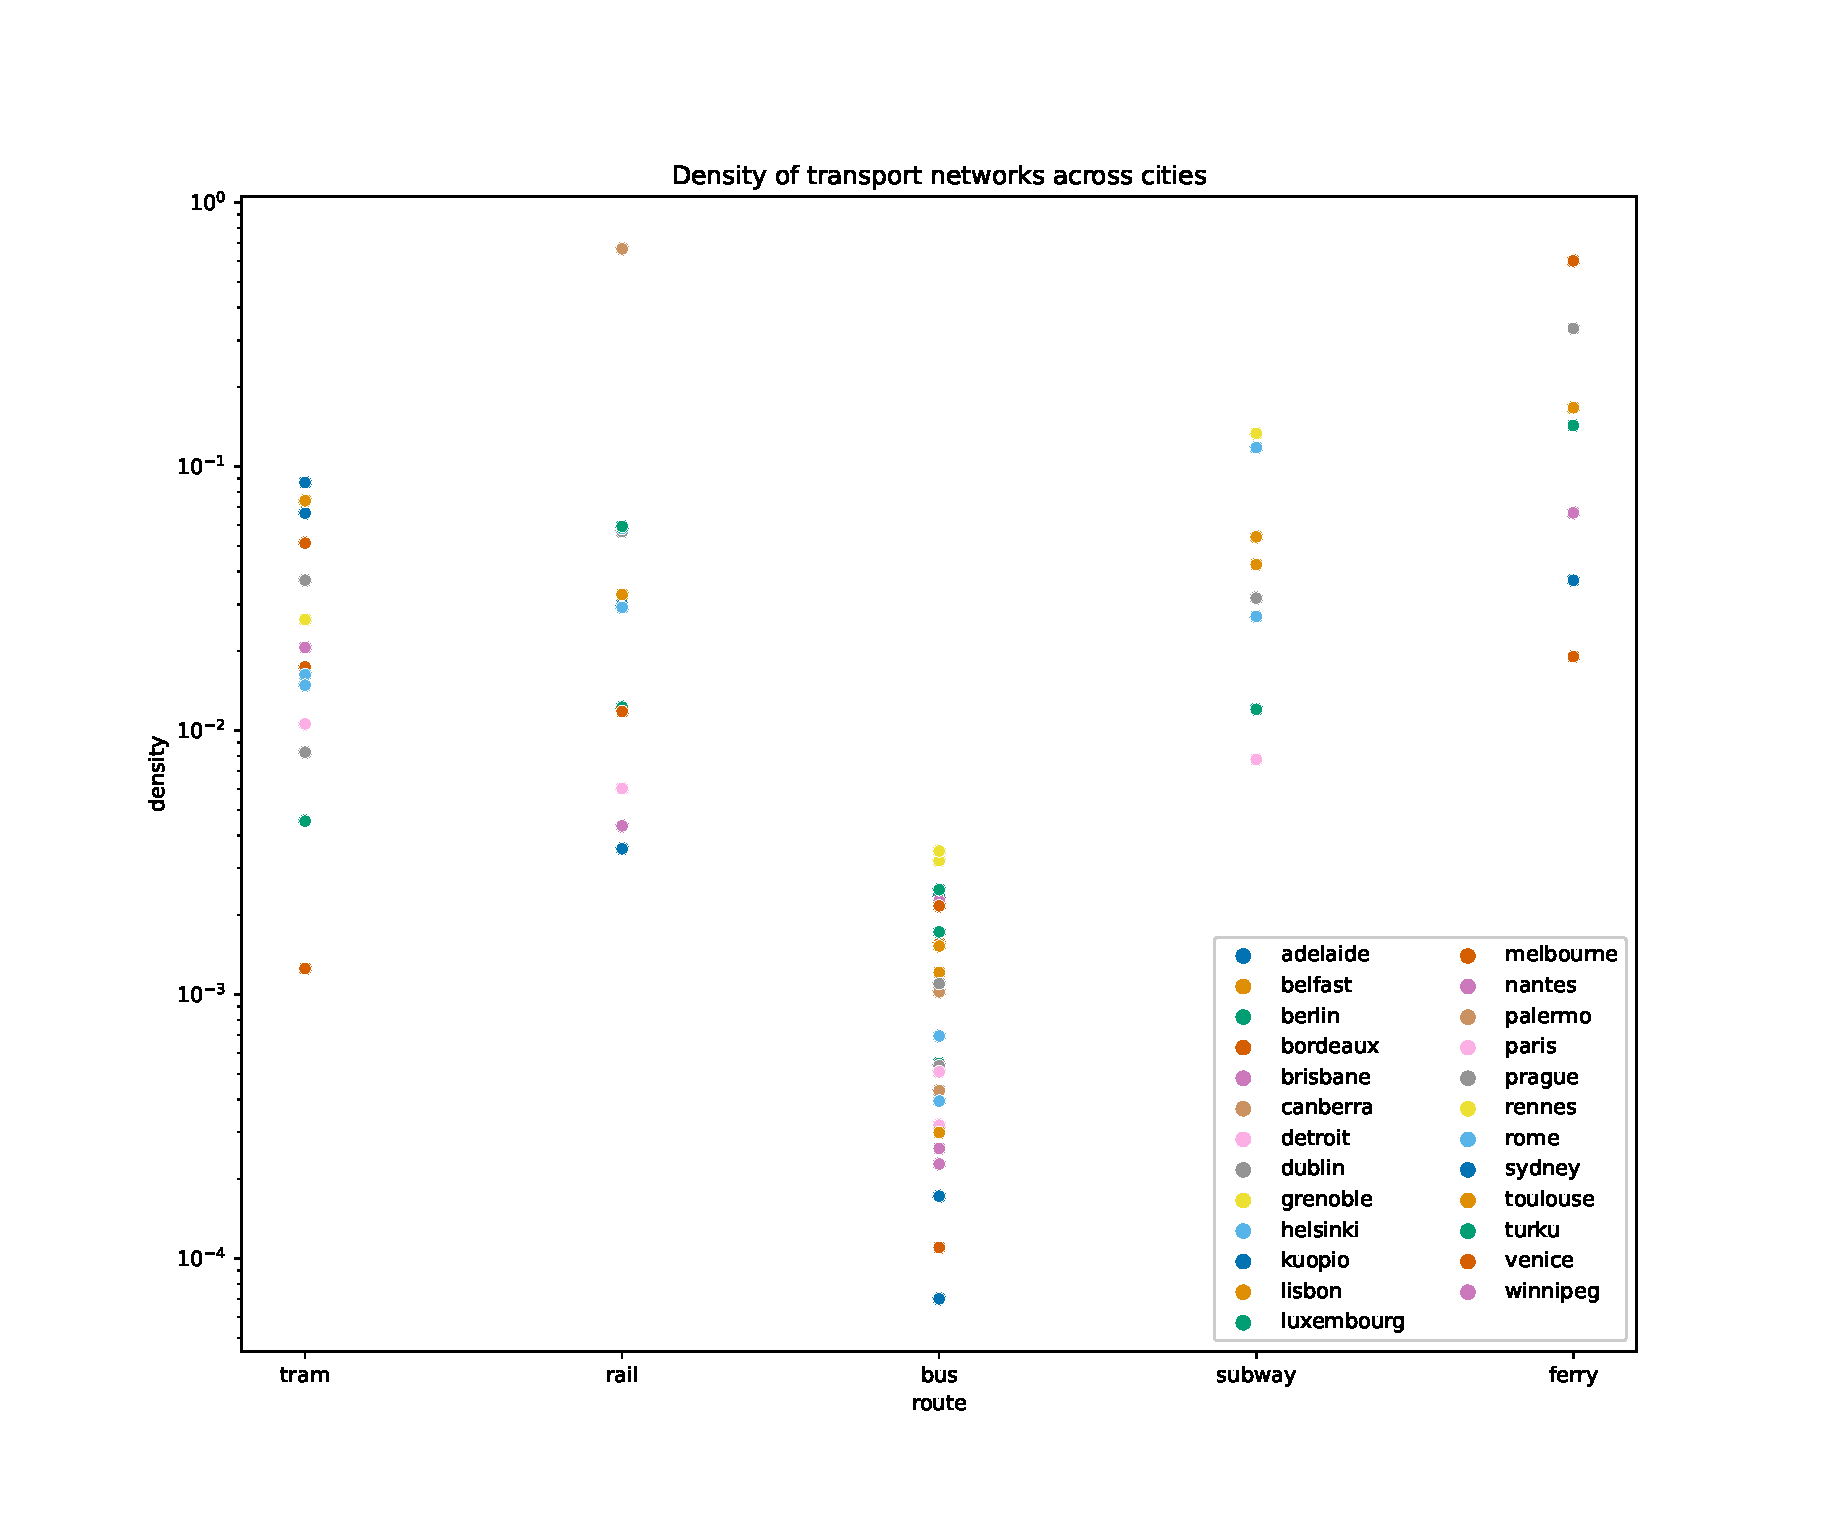
\includegraphics[width=\columnwidth]{images/city_route_density_distribution.eps}}
\caption{Transport Network Density Distribution in each city}
\label{net-density}
\end{center}
\vskip -0.3in
\end{figure}

\cref{net-density} shows the density of each mode of transport except for not strongly connected ones. The density of bus networks is very low compared to other networks implying fewer connections between stops, which makes travel difficult between different locations within the network. However, buses might provide last-mile connectivity and go around shorter distances in a limited geographical area. The rail network follows the bus with ten times more density. Nevertheless, it still falls between 0.003 and an outlier value of 0.7. The outlier is the Canberra rail network with three nodes and four edges. The tram network has the third lowest density varying between 0.001 and 0.1. The subway networks have the second highest density roughly ten times less than that of the ferry network (with the highest density values lying in the range of 0.02 and 0.7). These results are expected as the transport networks do not connect all stops with the majority of the other stops and are sparse like other real-world networks \cite{frossard_2023a}. 

Figures \ref{in-deg} and \ref{out-deg} show the in-degree and the out-degree distributions for various modes of transport in each city. The in-degree distribution follows a very similar pattern to the out-degree distribution. The distributions highlight many nodes with low degrees and a few with high degrees, making it difficult to model them by a random network model. The median value of city networks' average node degrees was calculated as 2.03, probably implying that each stop connects to two other stops. An interesting observation from the degree distribution is the nodes with zero in and out degrees. Although it is not completely clear it happens in the dataset, digging into the data can give some reasons. Firstly, there are many stops (especially in bus networks) with different names on either side of the road. Another reason could be that the public transport vehicles did not make the trip through those nodes during the data collection period, or they travelled empty to the start station.

\begin{figure}[ht]
\vskip -0.1in
\begin{center}
\centerline{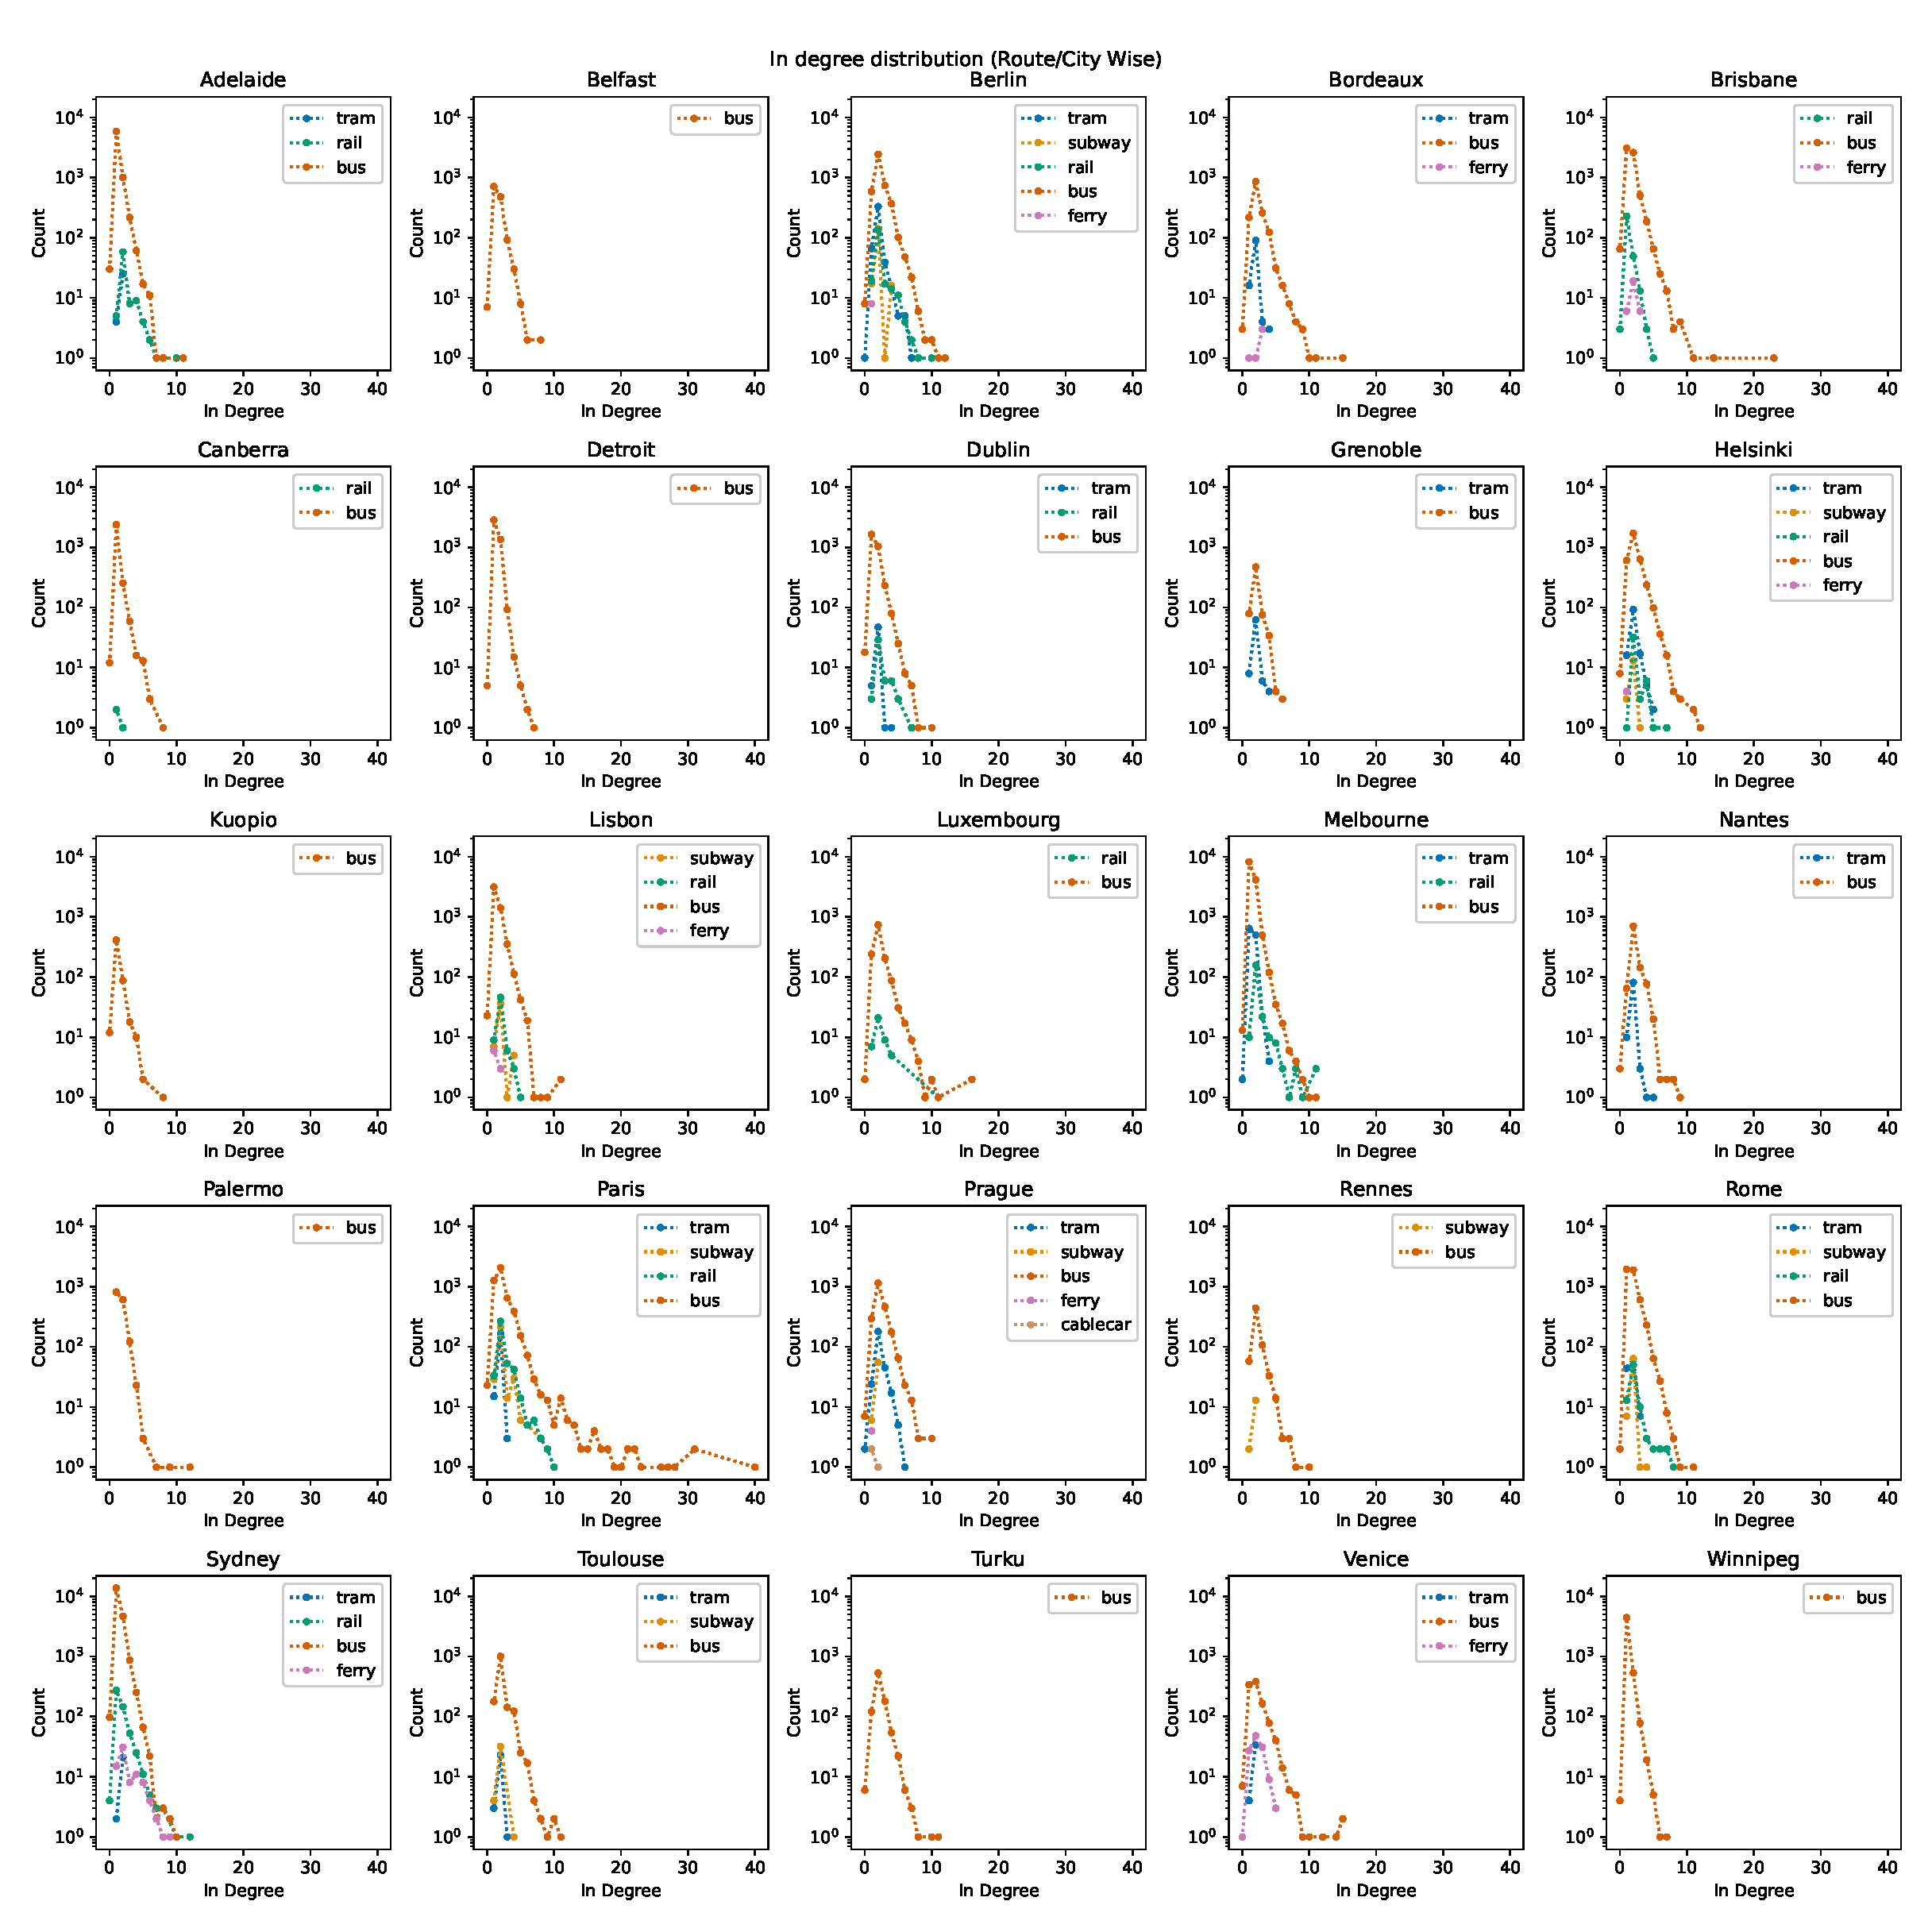
\includegraphics[width=\columnwidth]{images/in_deg_distribution.eps}}
\caption{Node In-Degree Distribution in each city}
\label{in-deg}
\end{center}
\vskip -0.3in
\end{figure}

\begin{figure}[ht]
\vskip -0.1in
\begin{center}
\centerline{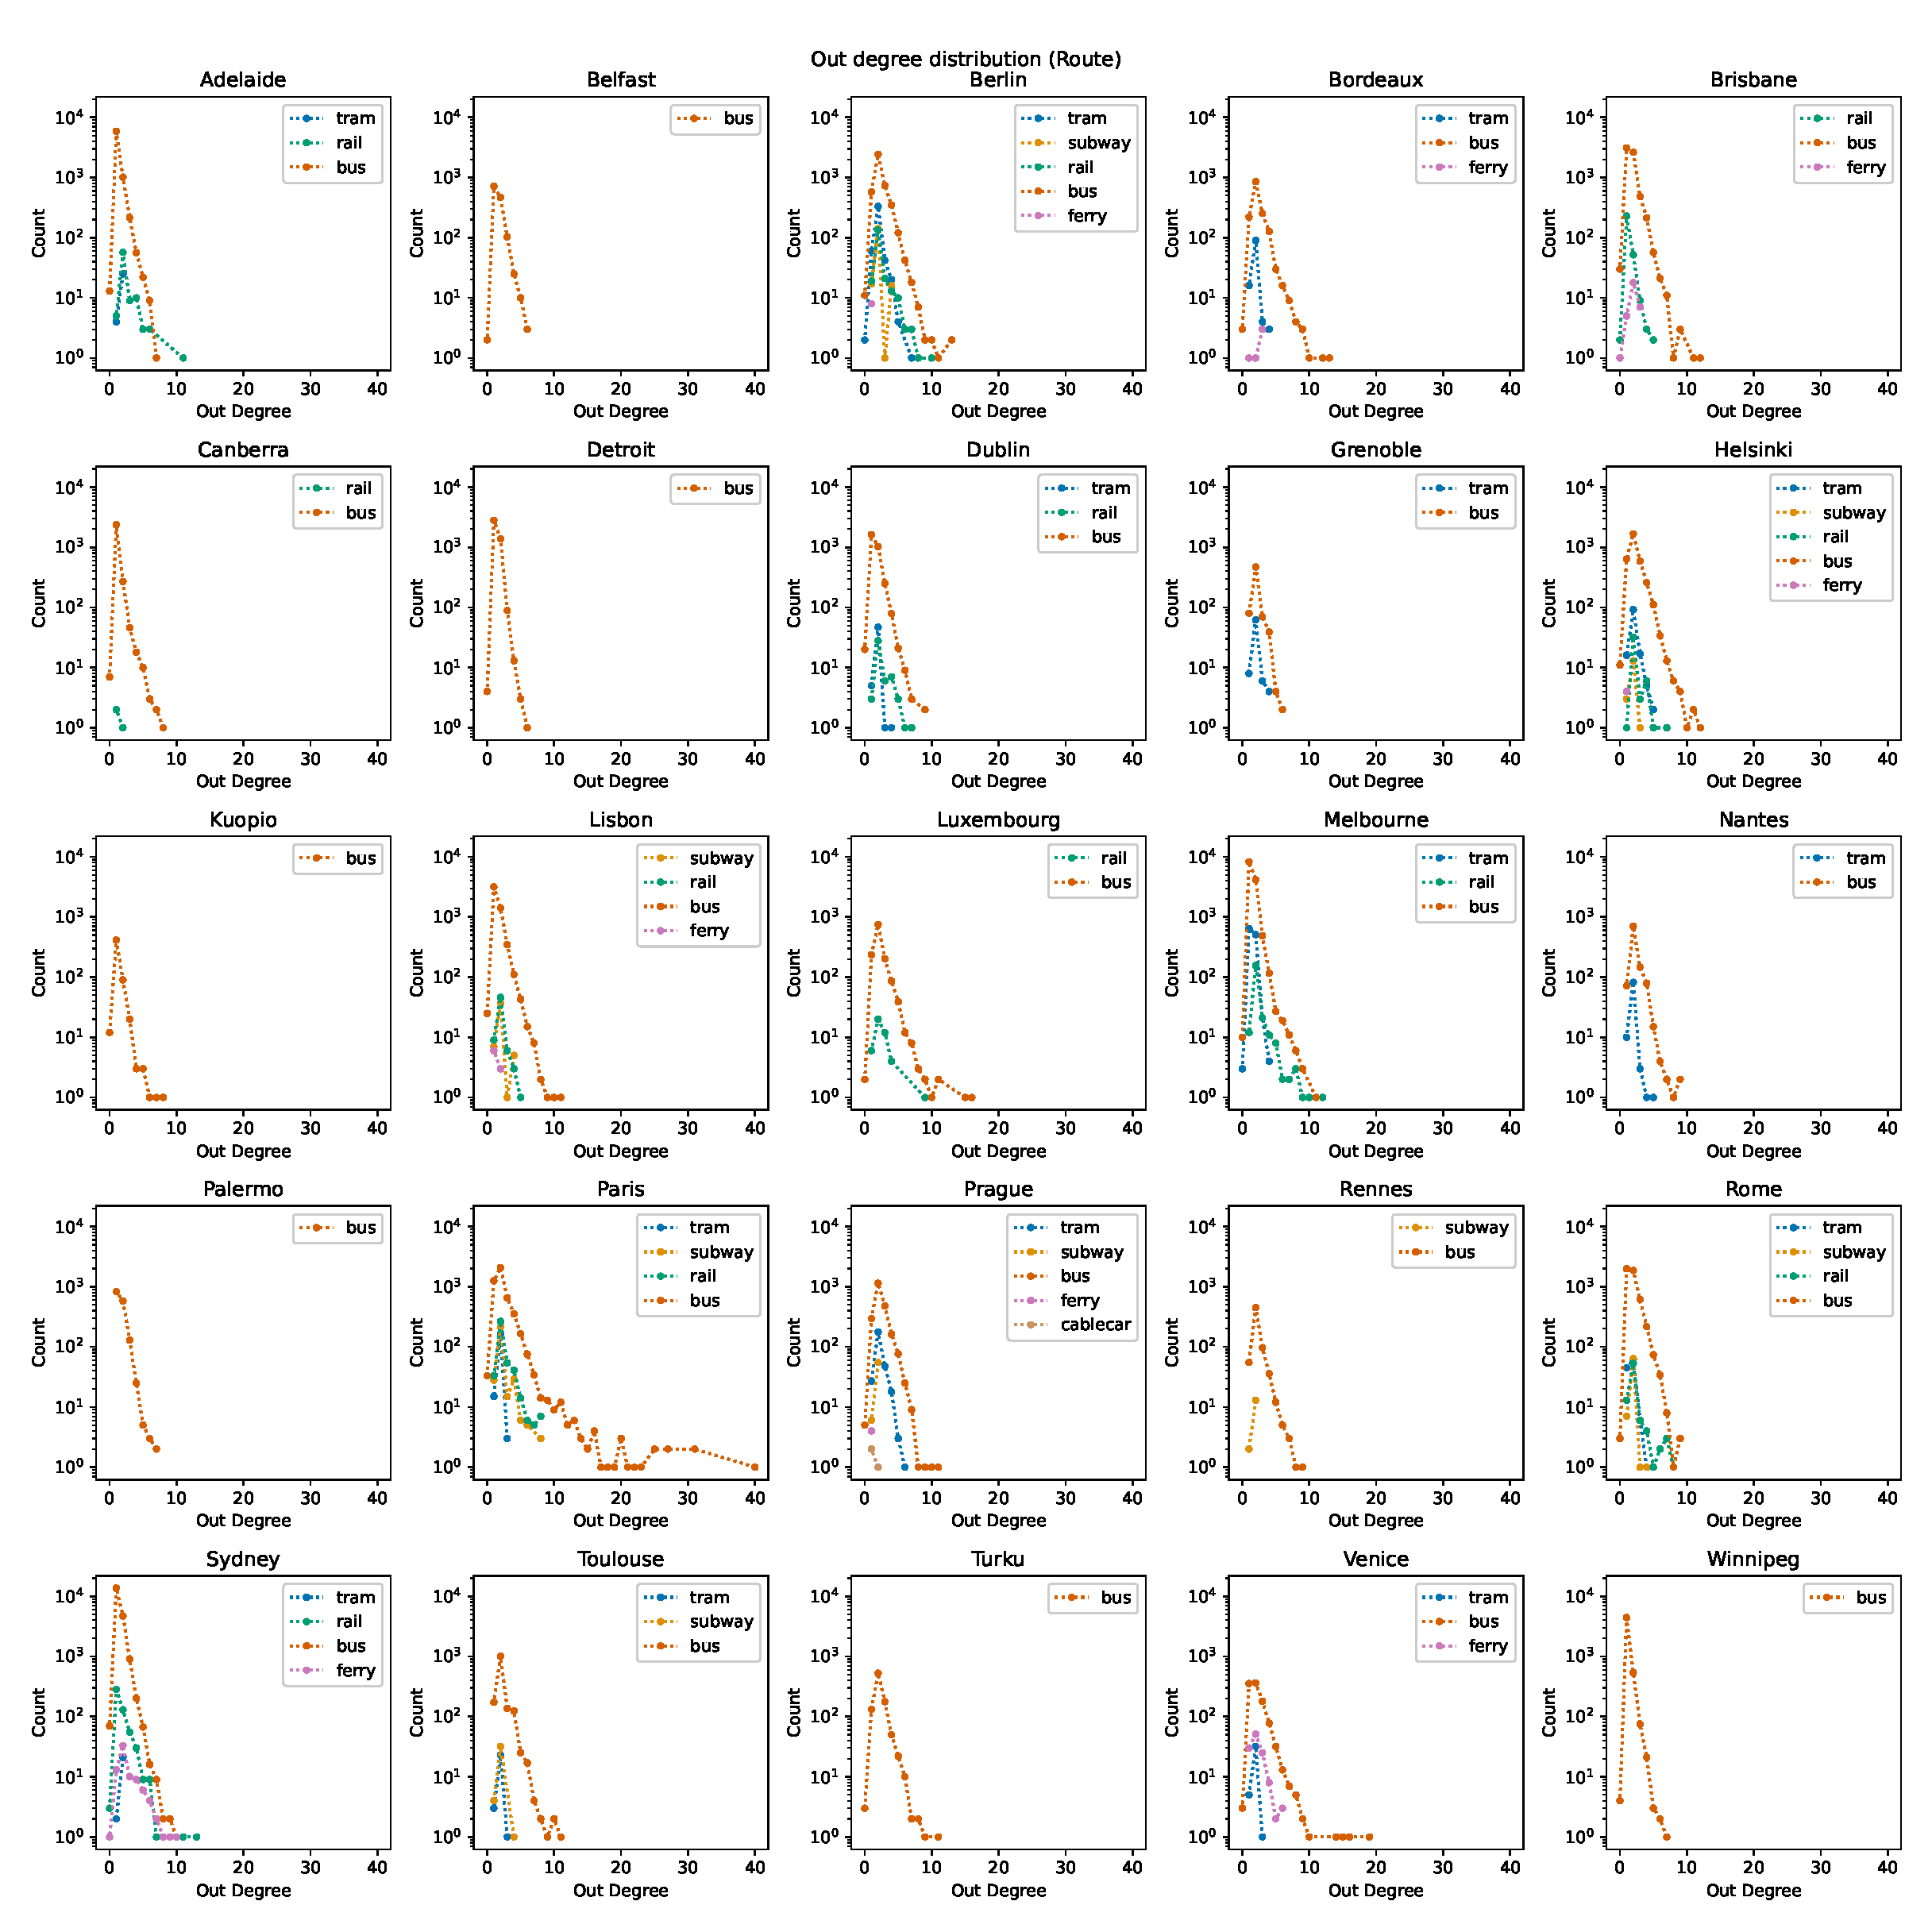
\includegraphics[width=\columnwidth]{images/out_deg_distribution.eps}}
\caption{Node Out-Degree Distribution in each city}
\label{out-deg}
\end{center}
\vskip -0.3in
\end{figure}

All the cities have around 1 minute of median travel time in the complete network except Detroit and Winnipeg, where it is half a minute and Paris and Prague, where it is nearly 2 minutes. However, on the individual transport mode level, people in Paris, Toulouse and Grenoble spend 2 minutes between two stops on average on the tram, and others spend around a minute to a minute and a half. For the subways, Helsinki has the highest time of 1.9 minutes. People in Canberra spend 20 minutes between rail stations, followed by distantly second Luxembourg at 3.87 minutes. The average travel time between stops on the bus is around one minute. Only eight cities have ferries, and the average travel time between their piers is highest in Bordeaux (9.5 minutes), followed by Sydney (8.9 minutes), and only 2 minutes in Prague. Lastly, only Prague has a cable car with three nodes and an average duration of 1.5 minutes between the stops.

The Betweenness Centrality (BC) of the nodes calculated using the average duration between stops captures the relative importance of transfer nodes within the network. The results support the hypothesis that the nodes with the highest BC in the city network represent the transit stations between different modes of transport. Luxembourg, Gare Centrale in Luxembourg or S+U Gesundbrunnen Bhf (Berlin) in Berlin and Chatelet les Halles in Paris are a few examples that are either big transit stops or next to very busy ones. Some stations, such as those in Berlin's ferry network with three routes between two different nodes each, have zero centrality because the network has very few or disconnected nodes. 
\begin{figure}[ht]
\vskip -0.1in
\begin{center}
\centerline{
\includegraphics[width=\columnwidth]{images/winnipeg_BC.eps}}
\caption{Betweenness Centrality of nodes in Winnipeg}
\label{BC-winni}
\end{center}
\vskip -0.3in
\end{figure} 

\begin{figure}[ht]
\vskip -0.1in
\begin{center}
\centerline{
\includegraphics[width=\columnwidth]{images/berlin_BC.eps}}
\caption{Betweenness Centrality of nodes in Berlin}
\label{BC-berlin}
\end{center}
\vskip -0.3in
\end{figure}

\cref{BC-winni} visualises the network in Winnipeg with nodes colour coded using the BC values. The nodes in yellow have the highest BC and are close to the city centre. \cref{BC-berlin} visualises the Berlin network, and nodes on the city's periphery and centre have the highest BC. Further examination revealed that they are the transit stations between different lines of the Berlin S-Bahn, regional and long-distance trains of the German train network. In a no longer online document \cite{DB_kategorien}, German's national rail company categorises six stations among the top ten nodes of Berlin, having the highest BC, as category 1 and 2 stations. These highly classified stations have heavy and efficient infrastructure, are frequented heavily and serve as critical transfer points.

% \begin{figure}[ht]
% \vskip -0.1in
% \begin{center}
% \centerline{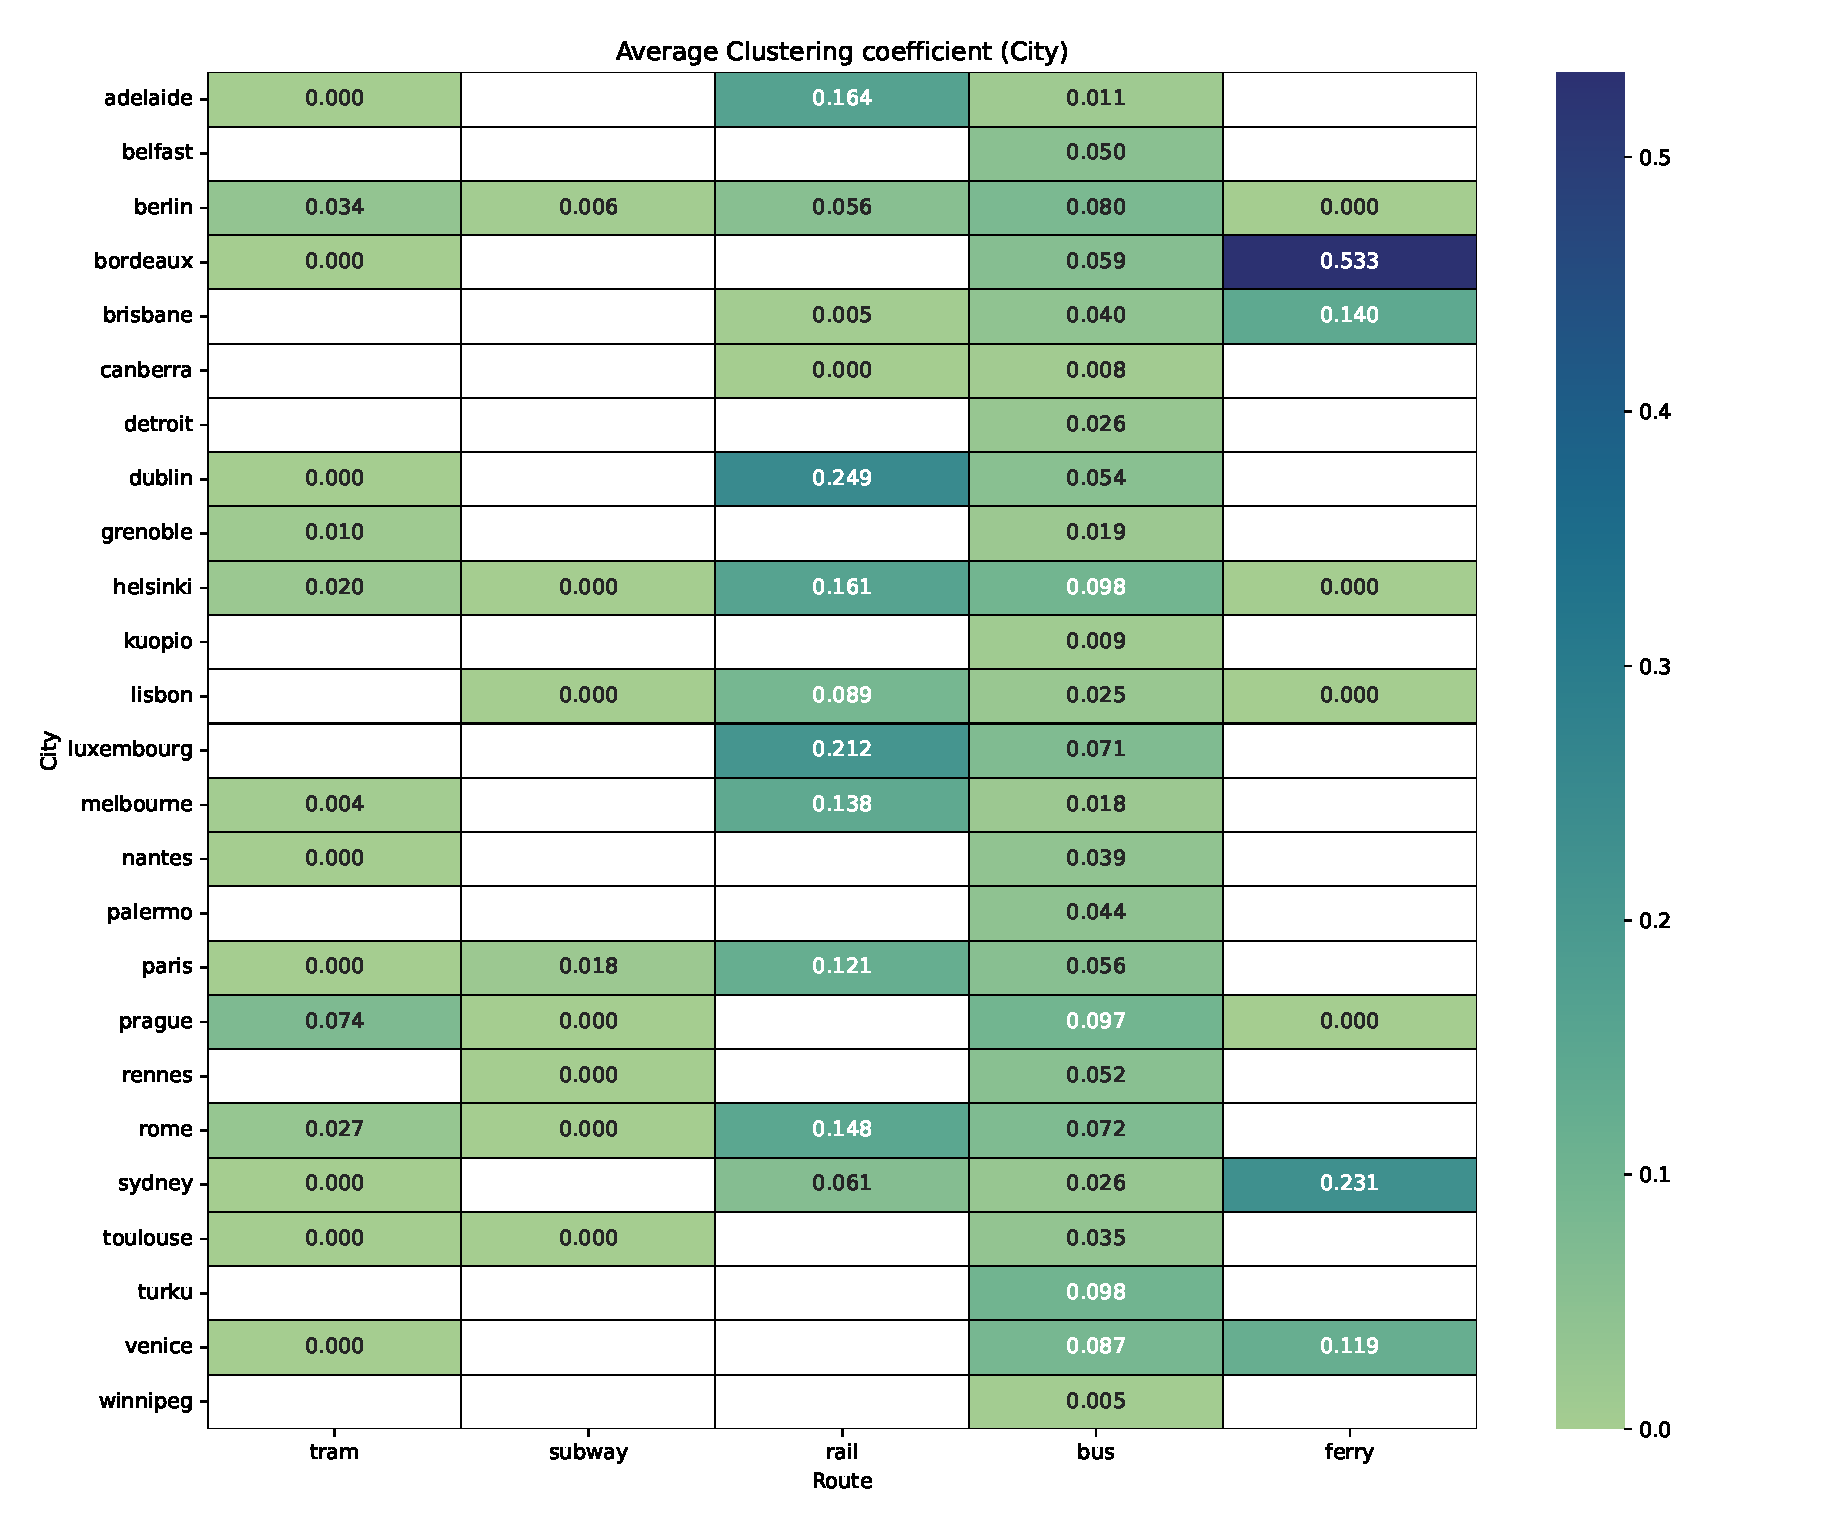
\includegraphics[width=\columnwidth]{images/clustering_coeff.eps}}
% \caption{Average Clustering Coefficient for each mode of transport in each city}
% \label{acc}
% \end{center}
% \vskip -0.3in
% \end{figure}

For transport networks, Average Clustering Coefficient (ACC) can provide insight into the local connectivity of the network and the extent to which transportation nodes are connected \cite{frossard_2023a}. A high average clustering coefficient indicates that the nodes tend to be densely connected, forming clusters or hubs. A low average clustering coefficient could imply that transportation nodes in the network are more sparsely connected, potentially leading to longer travel times or more complicated travel routes for travellers. In the 25 cities, almost all modes have low clustering coefficients, some even zero, indicating disconnected components like the Berlin ferry. The rail and bus modes have higher ACC, suggesting that they are better connected than the other modes of transport. Cities have one (or rarely two) modes with a high clustering coefficient.

Another parameter to measure the connectivity is the possibility of changing between different modes of transport, studied through the types of incoming and outgoing edges of a node. A city can be well-connected if there are more opportunities to switch between different modes of transport. In other words, a higher number of nodes with multiple transportation options passing through them indicates a well-connected transport network. However, this analysis does not fully apply to cities like Belfast, Detroit, Kuopio, Palermo, Turku, and Winnipeg, as they only have bus transport. 

\begin{figure}[ht]
\vskip -0.1in
\begin{center}
\centerline{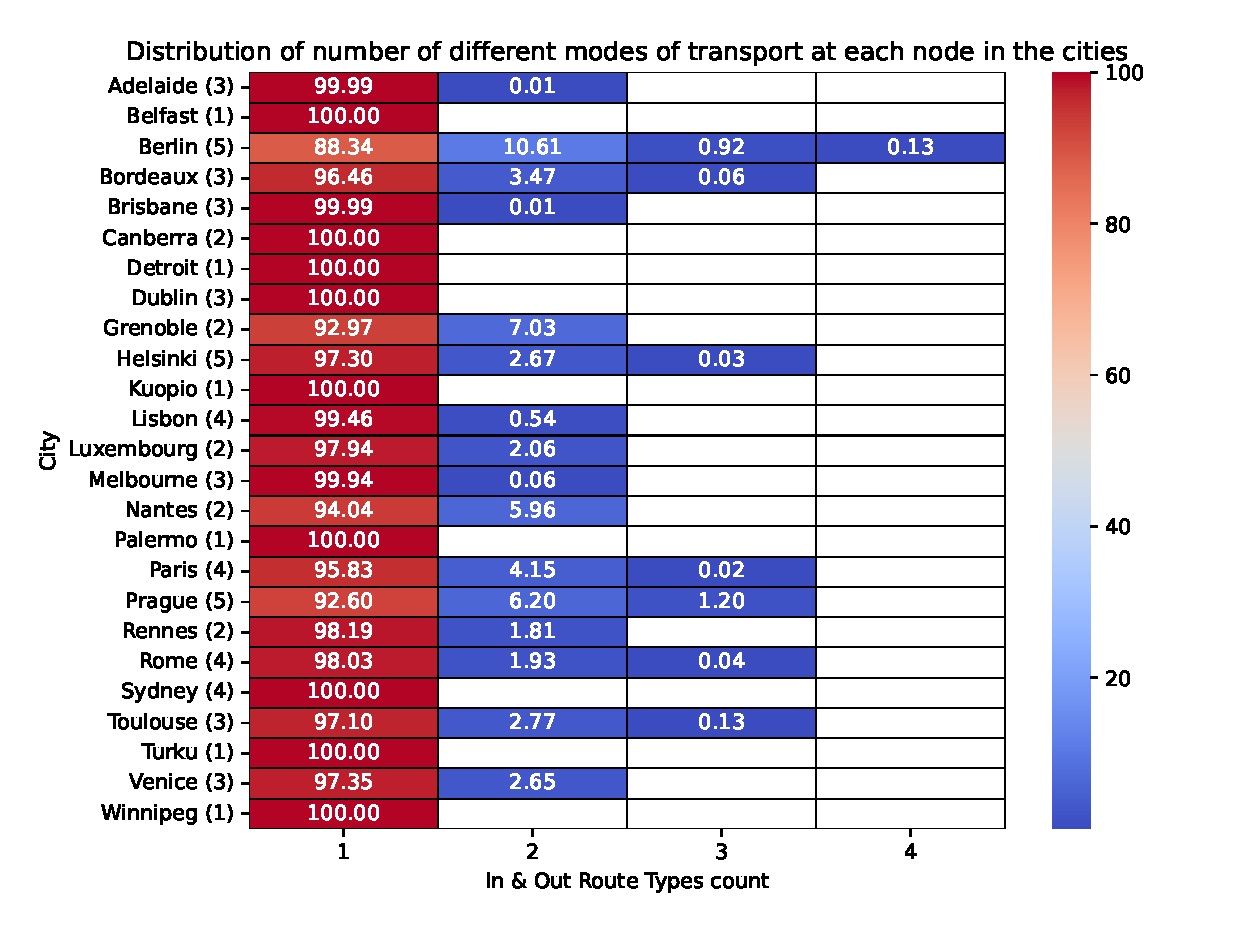
\includegraphics[width=\columnwidth]{images/intermodality_hm.eps}}
\caption{Number of modes of Transport at nodes in each city}
\label{intermode-node}
\end{center}
\vskip -0.3in
\end{figure}

\cref{intermode-node} shows the number of different transport modes at a stop on the x-axis and the number of nodes on the y-axis. For most cities, the distribution is skewed to the left, suggesting that most nodes accommodate only one mode. These cities have less interconnected transport networks, resulting in congestion at central stations where many people need to switch public transport vehicles. Adelaide, Brisbane, Canberra, Dublin, Melbourne and Sydney belong to this category, although Adelaide, Melbourne and Sydney have three and four modes of transport, respectively. The second category comprises cities with moderately connected networks, such as Bordeaux, Helsinki, Lisbon, Luxembourg, Paris, Rennes, Rome and Venice. In these cities, a relatively higher number of nodes connect with more than one or two modes of transport. Lastly, the well-connected cities include Berlin, Grenoble, Nantes, Prague and Toulouse. These cities have a higher proportion of nodes connecting to diverse transportation modes allowing passengers to disperse across multiple stations, facilitating ease of movement. It's important to note that this analysis solely focuses on theoretical connectivity and does not account for factors like city area, population, or topography.

The strongly connected components could represent areas with dense connections, where passengers can easily travel within the component but may have more difficulty reaching nodes outside of it \cite{frossard_2023b}. The weakly connected components may indicate areas that are not well connected or have limited accessibility. Strong components potentially represent the full-service routes, and weak components represent the somewhat connected service routes. The results show Adelaide, Brisbane, Kuopio, Lisbon, and Sydney have more than 100 strongly connected components and a few with more than 50. Weakly connected components were less than 7 in all cities except Sydney (18).

% \begin{figure}[ht]
% \vskip -0.1in
% \begin{center}
% \centerline{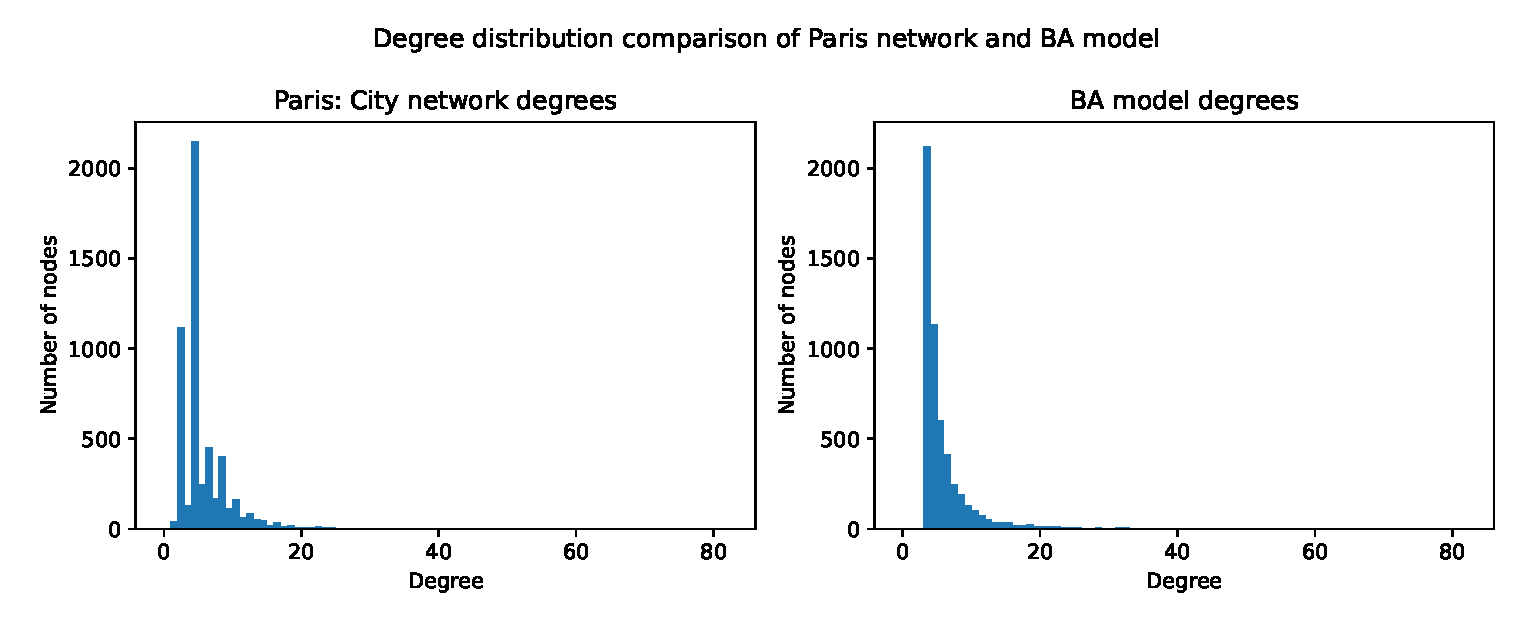
\includegraphics[width=\columnwidth]{images/paris_BA.eps}}
% \caption{Degree distribution comparison of Paris network and BA model}
% \label{paris-BA}
% \end{center}
% \vskip -0.3in
% \end{figure}

% \begin{figure}[ht]
% \vskip -0.1in
% \begin{center}
% \centerline{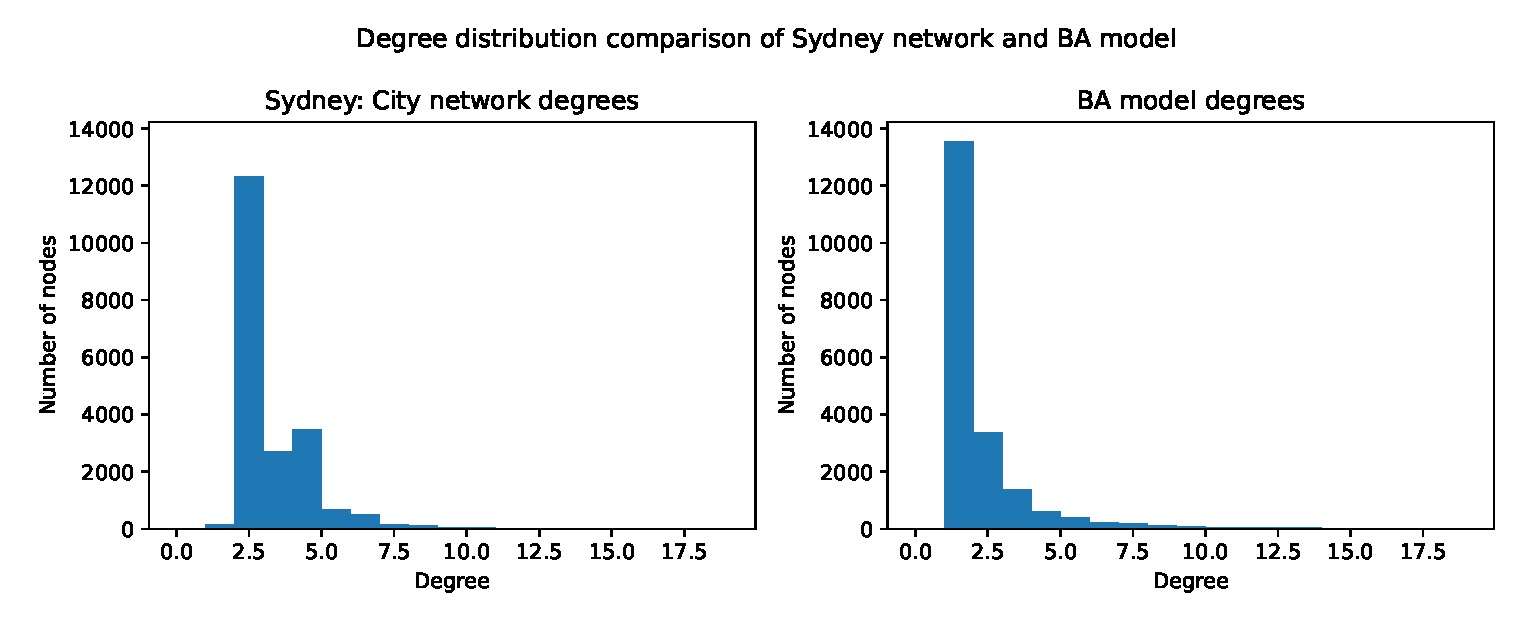
\includegraphics[width=\columnwidth]{images/sydney_BA.eps}}
% \caption{Degree distribution comparison of Sydney network and BA model}
% \label{sydney-BA}
% \end{center}
% \vskip -0.3in
% \end{figure}

% \begin{figure}[ht]
% \vskip -0.1in
% \begin{center}
% \centerline{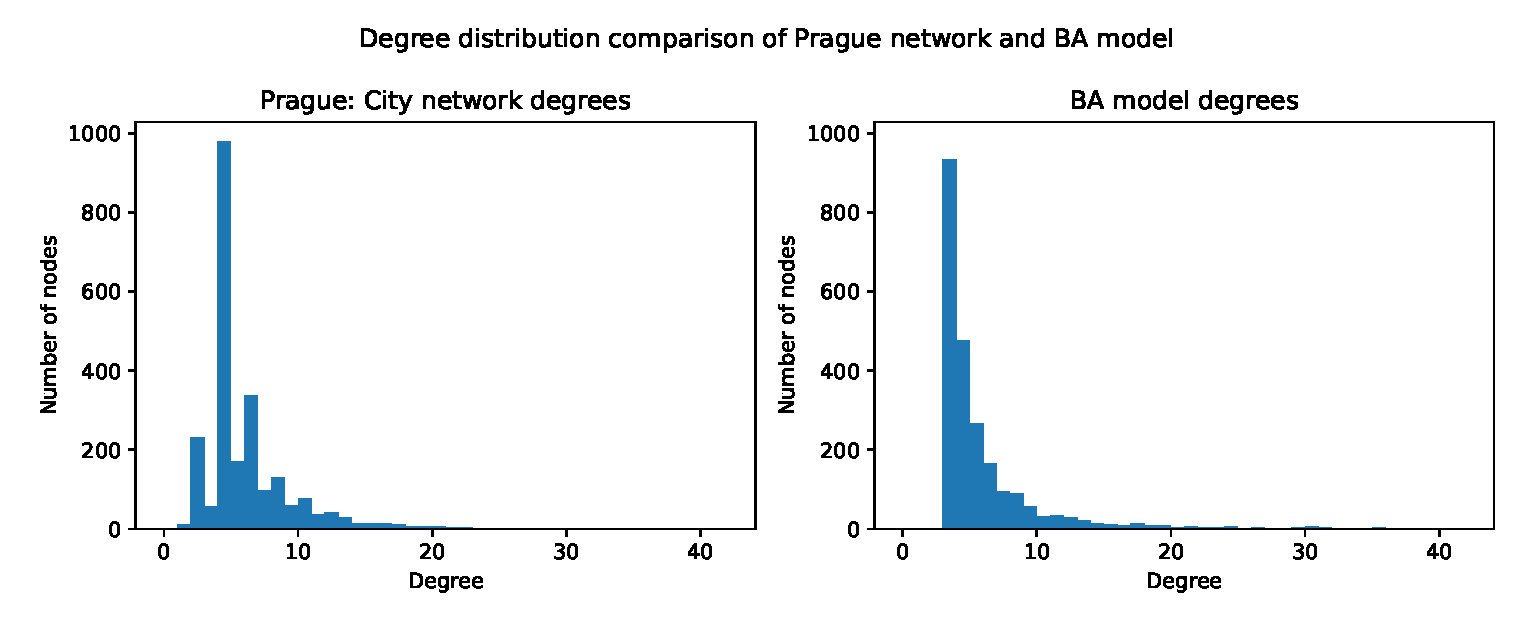
\includegraphics[width=\columnwidth]{images/prague_BA.eps}}
% \caption{Degree distribution comparison of Prague network and BA model}
% \label{prague-BA}
% \end{center}
% \vskip -0.3in
% \end{figure}

% \begin{figure}[ht]
% \vskip -0.1in
% \begin{center}
% \centerline{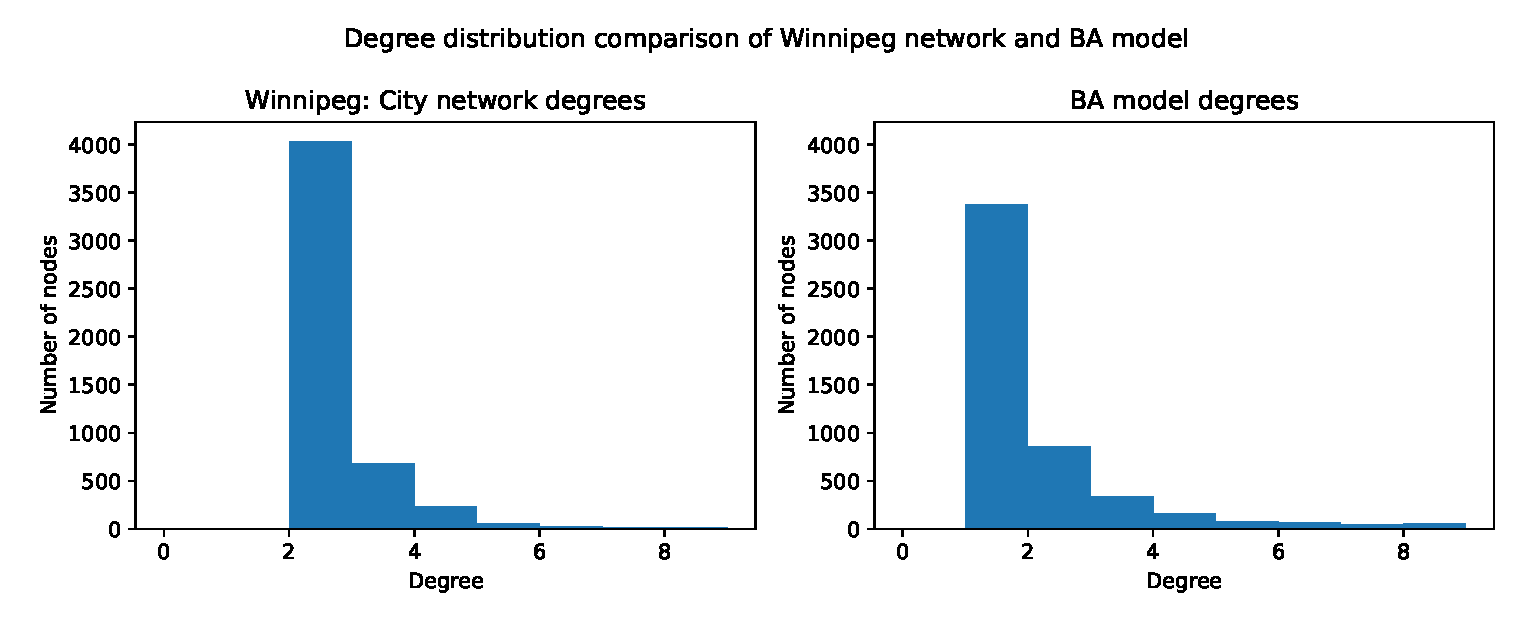
\includegraphics[width=\columnwidth]{images/winnipeg_BA.eps}}
% \caption{Degree distribution comparison of Winnipeg network and BA model}
% \label{winni-BA}
% \end{center}
% \vskip -0.3in
% \end{figure}

% (Figure \ref{sydney-BA} with 1000 starting nodes and Number of edges to attach from a new node to existing nodes set to half of average degree)
% (Figure \ref{prague-BA} with 500 starting nodes)

Lastly, the networks were modelled using the Barabasi-Albert (BA) model, which typically starts with an initial set of nodes and uses both growth and preferential attachment in developing the network \cite{frossard_2023d}. The results show that the BA model provides a reasonable approximation to model the nature of the degree distribution of the nodes in the network. For cities with a large number of nodes and edges, like Paris and Sydney, there is a steeper reduction in the number of nodes with the increase in the node degree. For smaller ones like Prague and Winnipeg, the decline is more gradual. Transport networks for larger cities may have a higher preferential attachment factor that is superlinear in terms of node degree \cite{frossard_2023d}. The BA model that applies a linear preferential attachment has a less steep reduction in the number of nodes for higher degrees. However, BA model is not best suited for these directed networks and does not consider the changing of stations and routes \cite{Barabási_2016}.

\subsection{Exploitation}
\label{exploitation}

This project attempts two exploitation tasks - edge prediction and label prediction. The former task aims to predict if a directed edge exists between two nodes, and the latter is to predict the type of edge(s) - the mode of transport - given that an edge already exists between two nodes. For both tasks, the experiments involve using two kinds of hand-crafted features and Node2Vec features. The first type of hand-crafted features uses the following individual node properties: in-degree centrality, out-degree centrality, betweenness centrality and Katz centrality. As the networks are directed, separate in and out-degree centrality was considered. The centrality measures were considered to capture the relative importance of each node in the network. The second type is shared properties of the two nodes: (1) the fraction of the number of shared incoming neighbours among all incoming neighbours between the nodes and (2) the fraction of the number of shared outgoing neighbours among all outgoing neighbours between the nodes. The node features of the source node were subtracted from the corresponding node features of the destination node to create edge features. The directedness of the edges in the network drove the decision to use subtraction in combining the node features to create edge features.

\subsubsection{Experiment Setup}
\label{setup}

Both prediction tasks involved training a logistic regression model with balanced class weights while using the hand-crafted and node2vec features for both prediction tasks. Informed by the results of the exploration phase, a different model was created for each transport type in each city with a 70:30 split of training and testing data while stratifying the split based on the targets. The reported F1 score is the weighted average score of each class. The Sydney bus network and Prague cable car network were excluded from the analysis due to repeated machine failures (most likely due to kernel memory issues) and as it was the only city with three stops in that category, respectively. The experiments employing the hand-crafted features involved three sub-experiments. First, only using the features derived from the node properties. Second, only using the common incoming and outgoing neighbour's features, and lastly, with all six of them. 

To mitigate the priors induced by the hand-crafted features, an alternative approach is considered through Node2Vec. The intuition behind the Node2vec embedding approach is to expect similar embeddings for nodes of the graph based on the local as well as the global view of the node neighbourhood \cite{grover2016node2vec}. The approach interpolates among the Breadth-first search as well as the Depth-first search algorithms with tuning parameters $p$ and $q$ to control the nature and extent of this neighbourhood to constrain the random walk exploration/generation. Both of them were set to 1, and they represent \cite{grover2016node2vec}:
\begin{enumerate}
    \item $p$ - Return parameter controls the likelihood of immediately revisiting a node in the random walk.
    \item $q$ - The in-out parameter controls how fast the next walk explores or leaves the neighbourhood of a starting node.
\end{enumerate}

\subsubsection{Edge Prediction}
\label{edge-pred}
Edge features were created for all pair of nodes in the network, to train the edge prediction model. Thus, each network with $N$ nodes has $N(N-1)$ edges in the training set with the features as one of the four possible hand-crafted features and a label 1 if the edge exists in the network or 0 if it does not. 

\begin{figure}[ht]
\vskip -0.1in
\begin{center}
\centerline{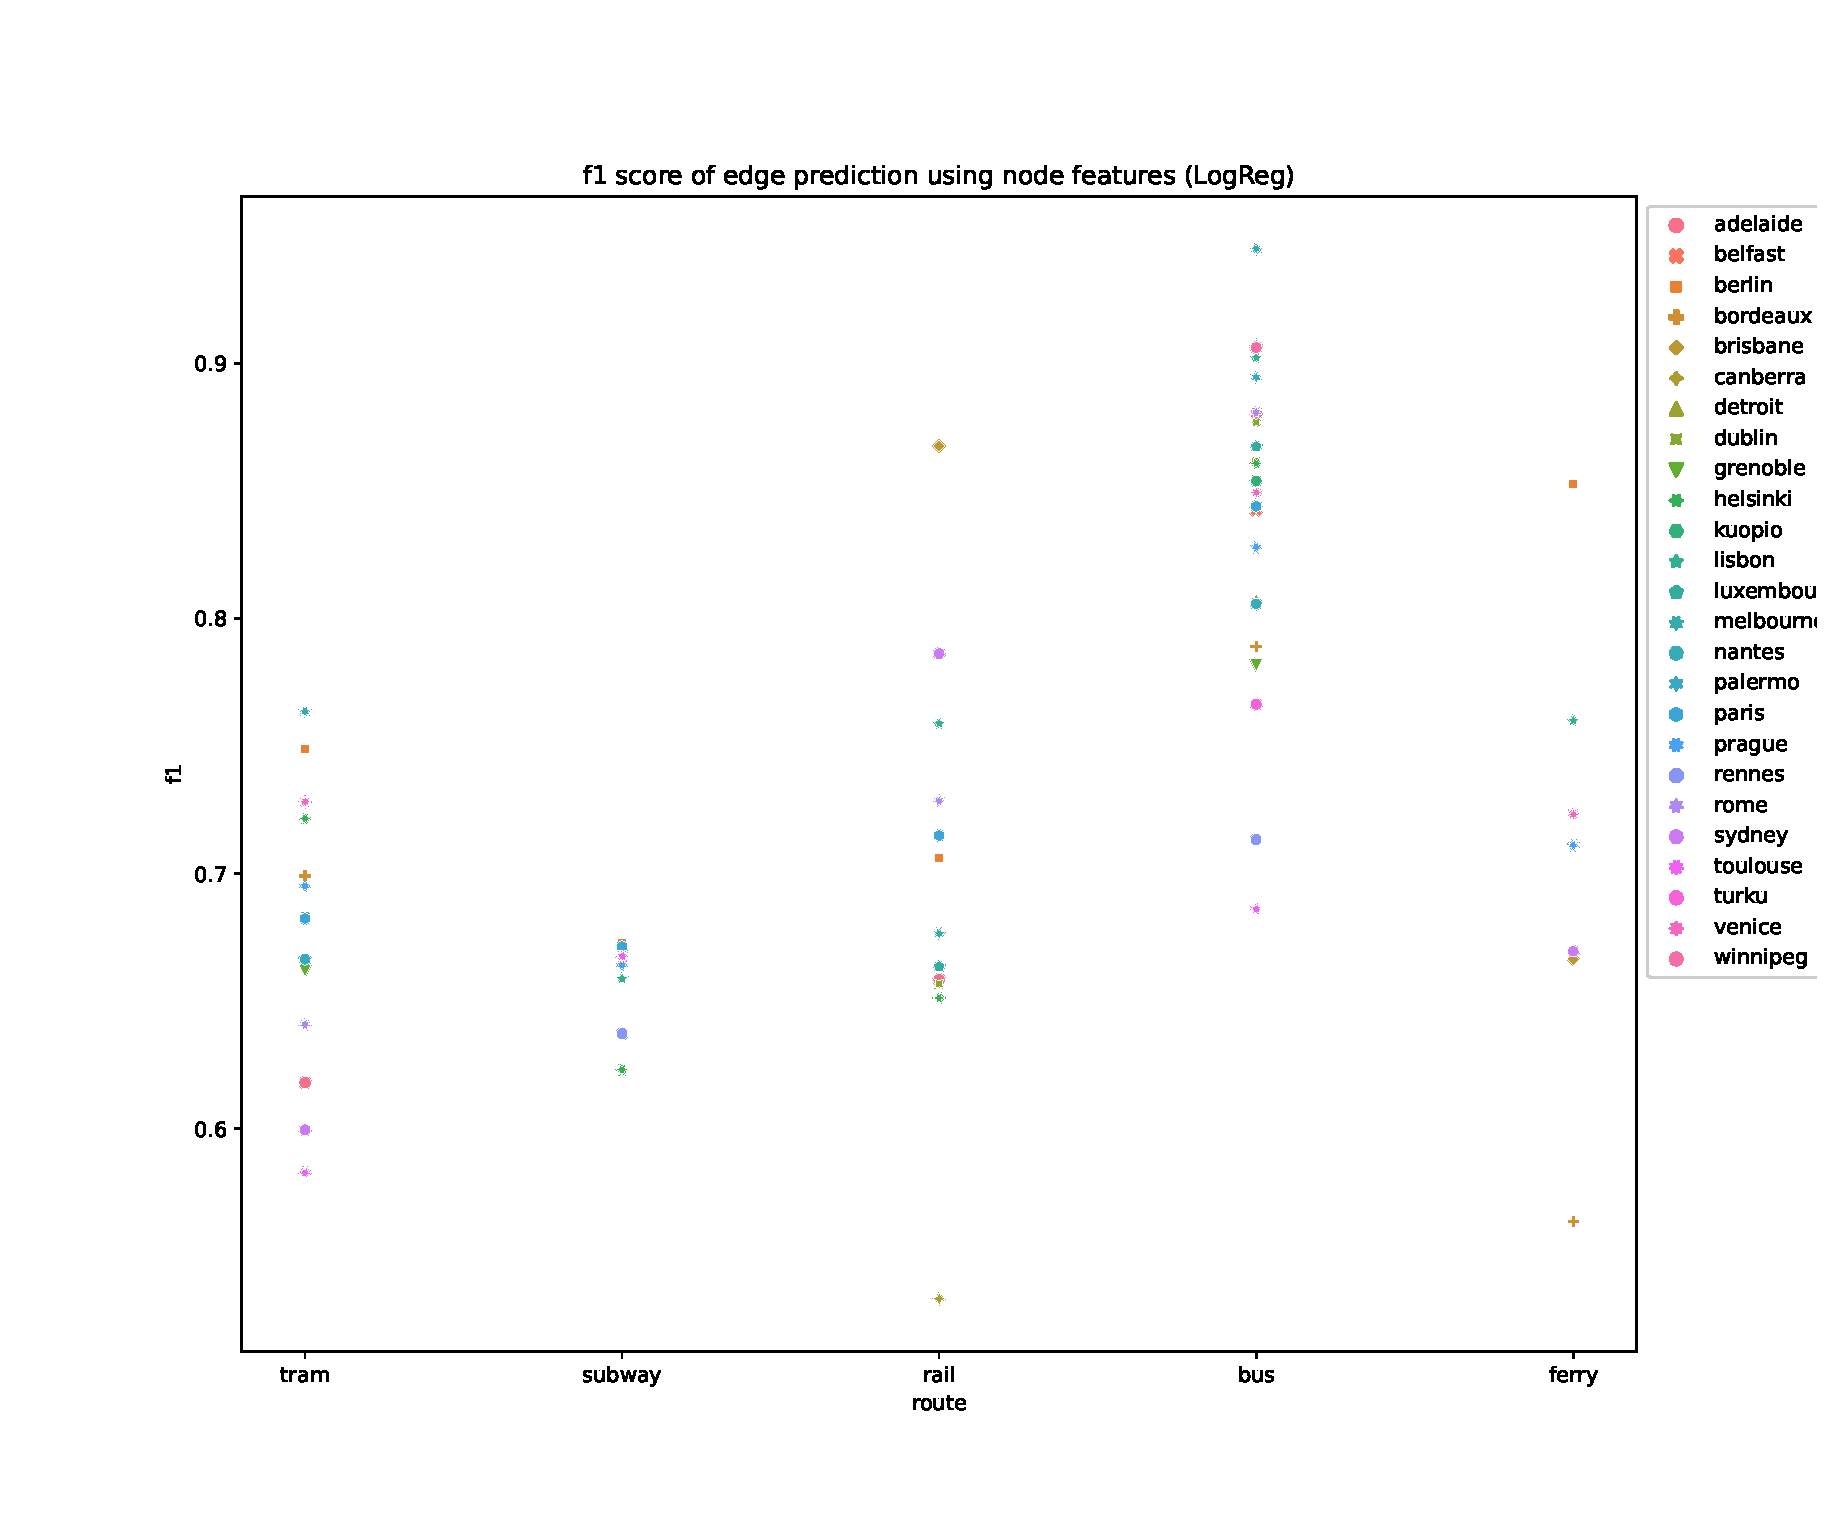
\includegraphics[width=\columnwidth]{images/edge-pred-node.eps}}
\caption{F1 score of edge prediction using node properties}
\label{edge-pred-node_fig}
\end{center}
\vskip -0.3in
\end{figure}

\begin{figure}[ht]
\vskip -0.1in
\begin{center}
\centerline{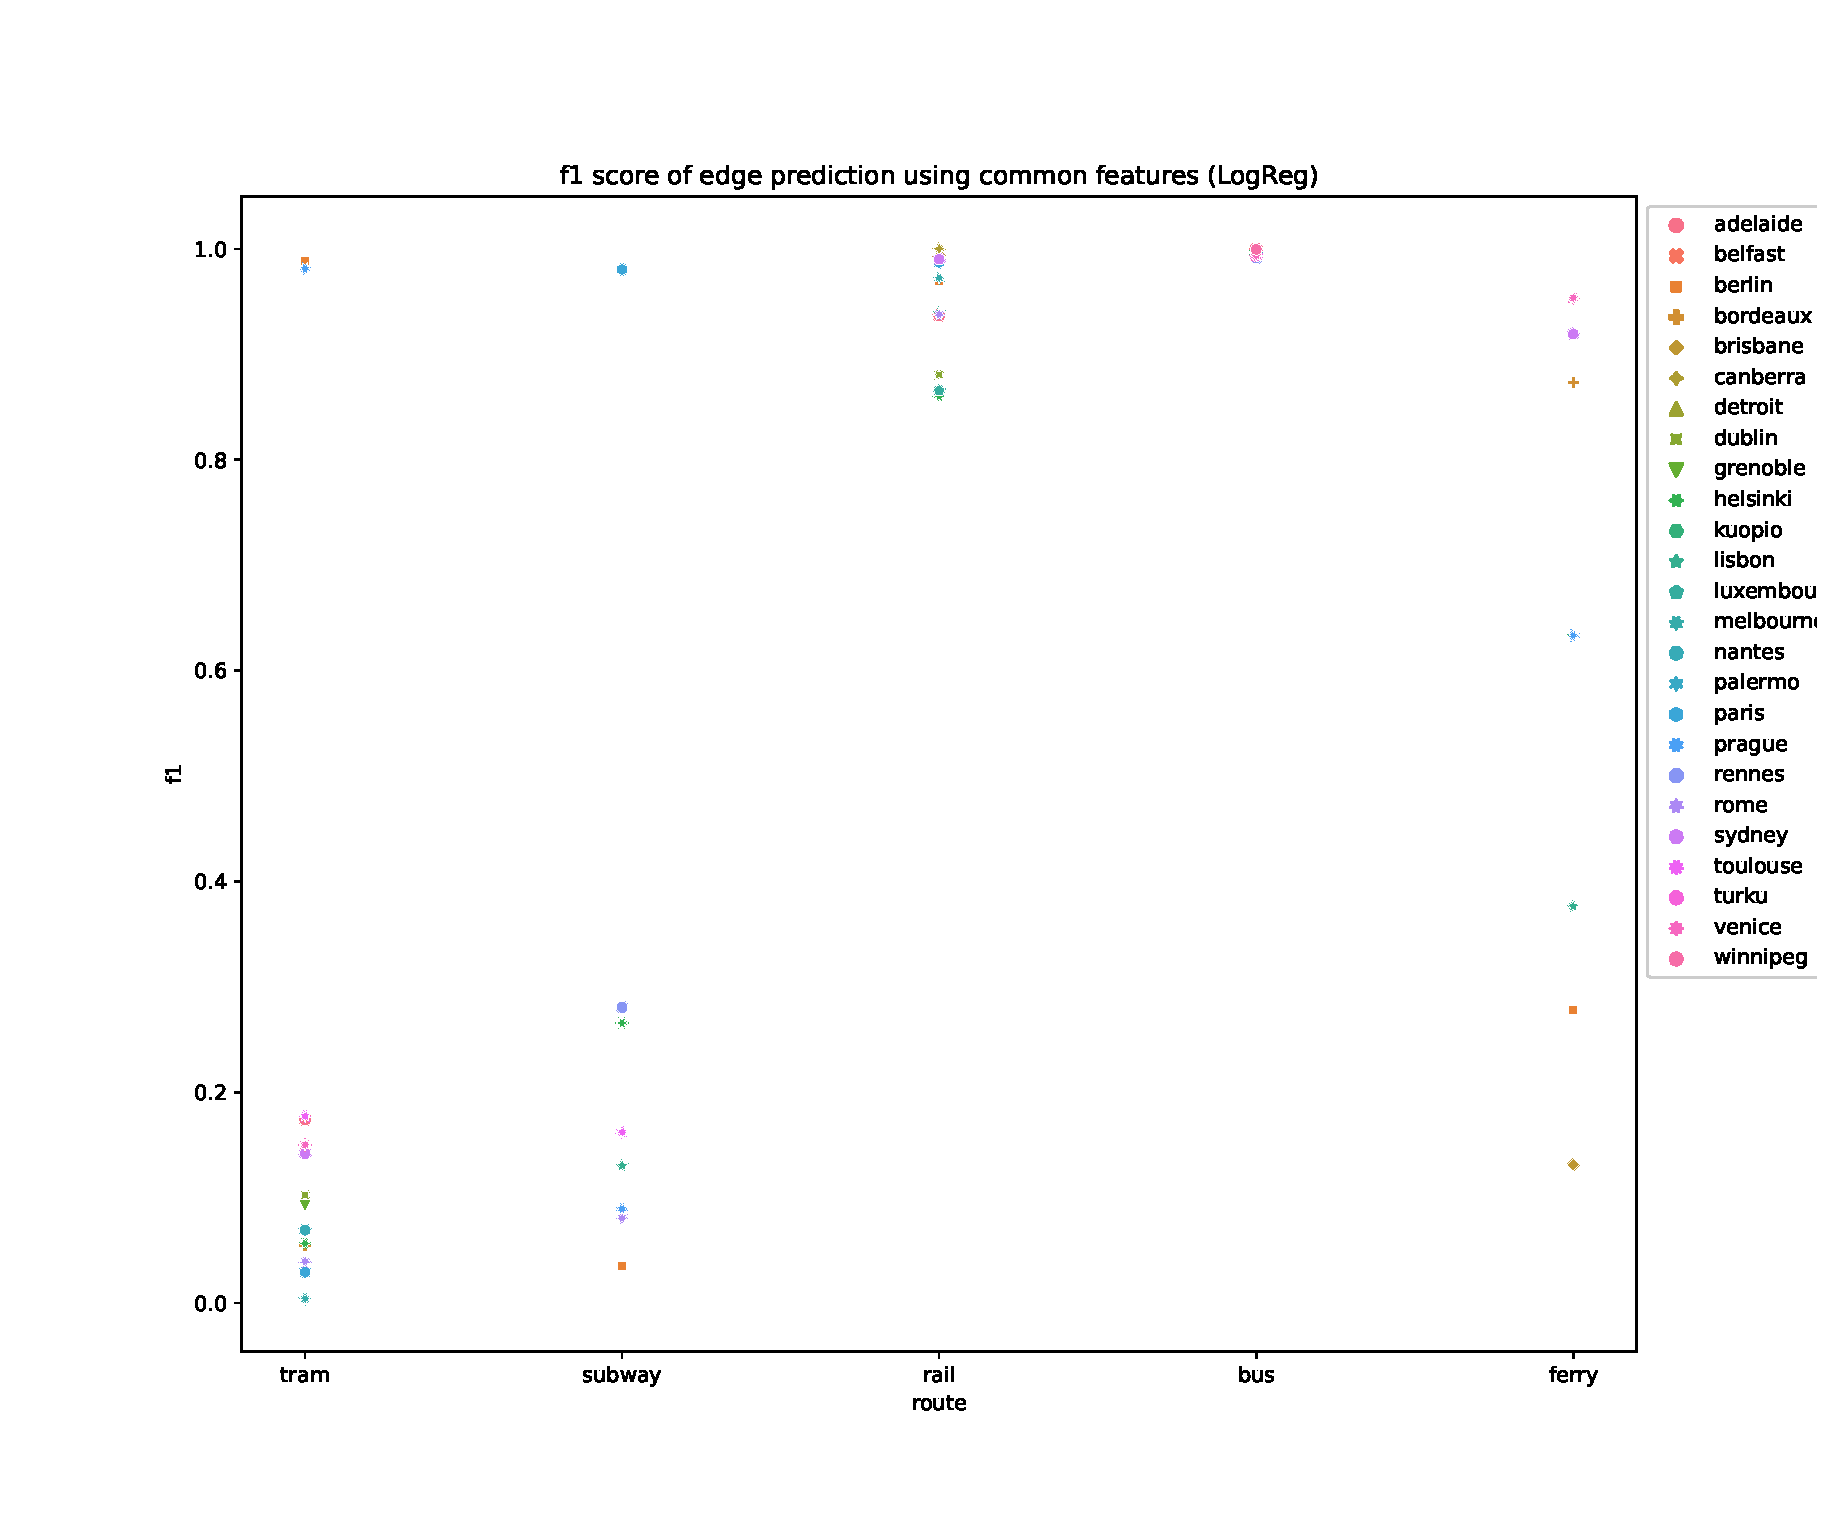
\includegraphics[width=\columnwidth]{images/edge-pred-commono.eps}}
\caption{F1 score of edge prediction using common properties}
\label{edge-pred-common_fig}
\end{center}
\vskip -0.3in
\end{figure}

\begin{figure}[ht]
\vskip -0.1in
\begin{center}
\centerline{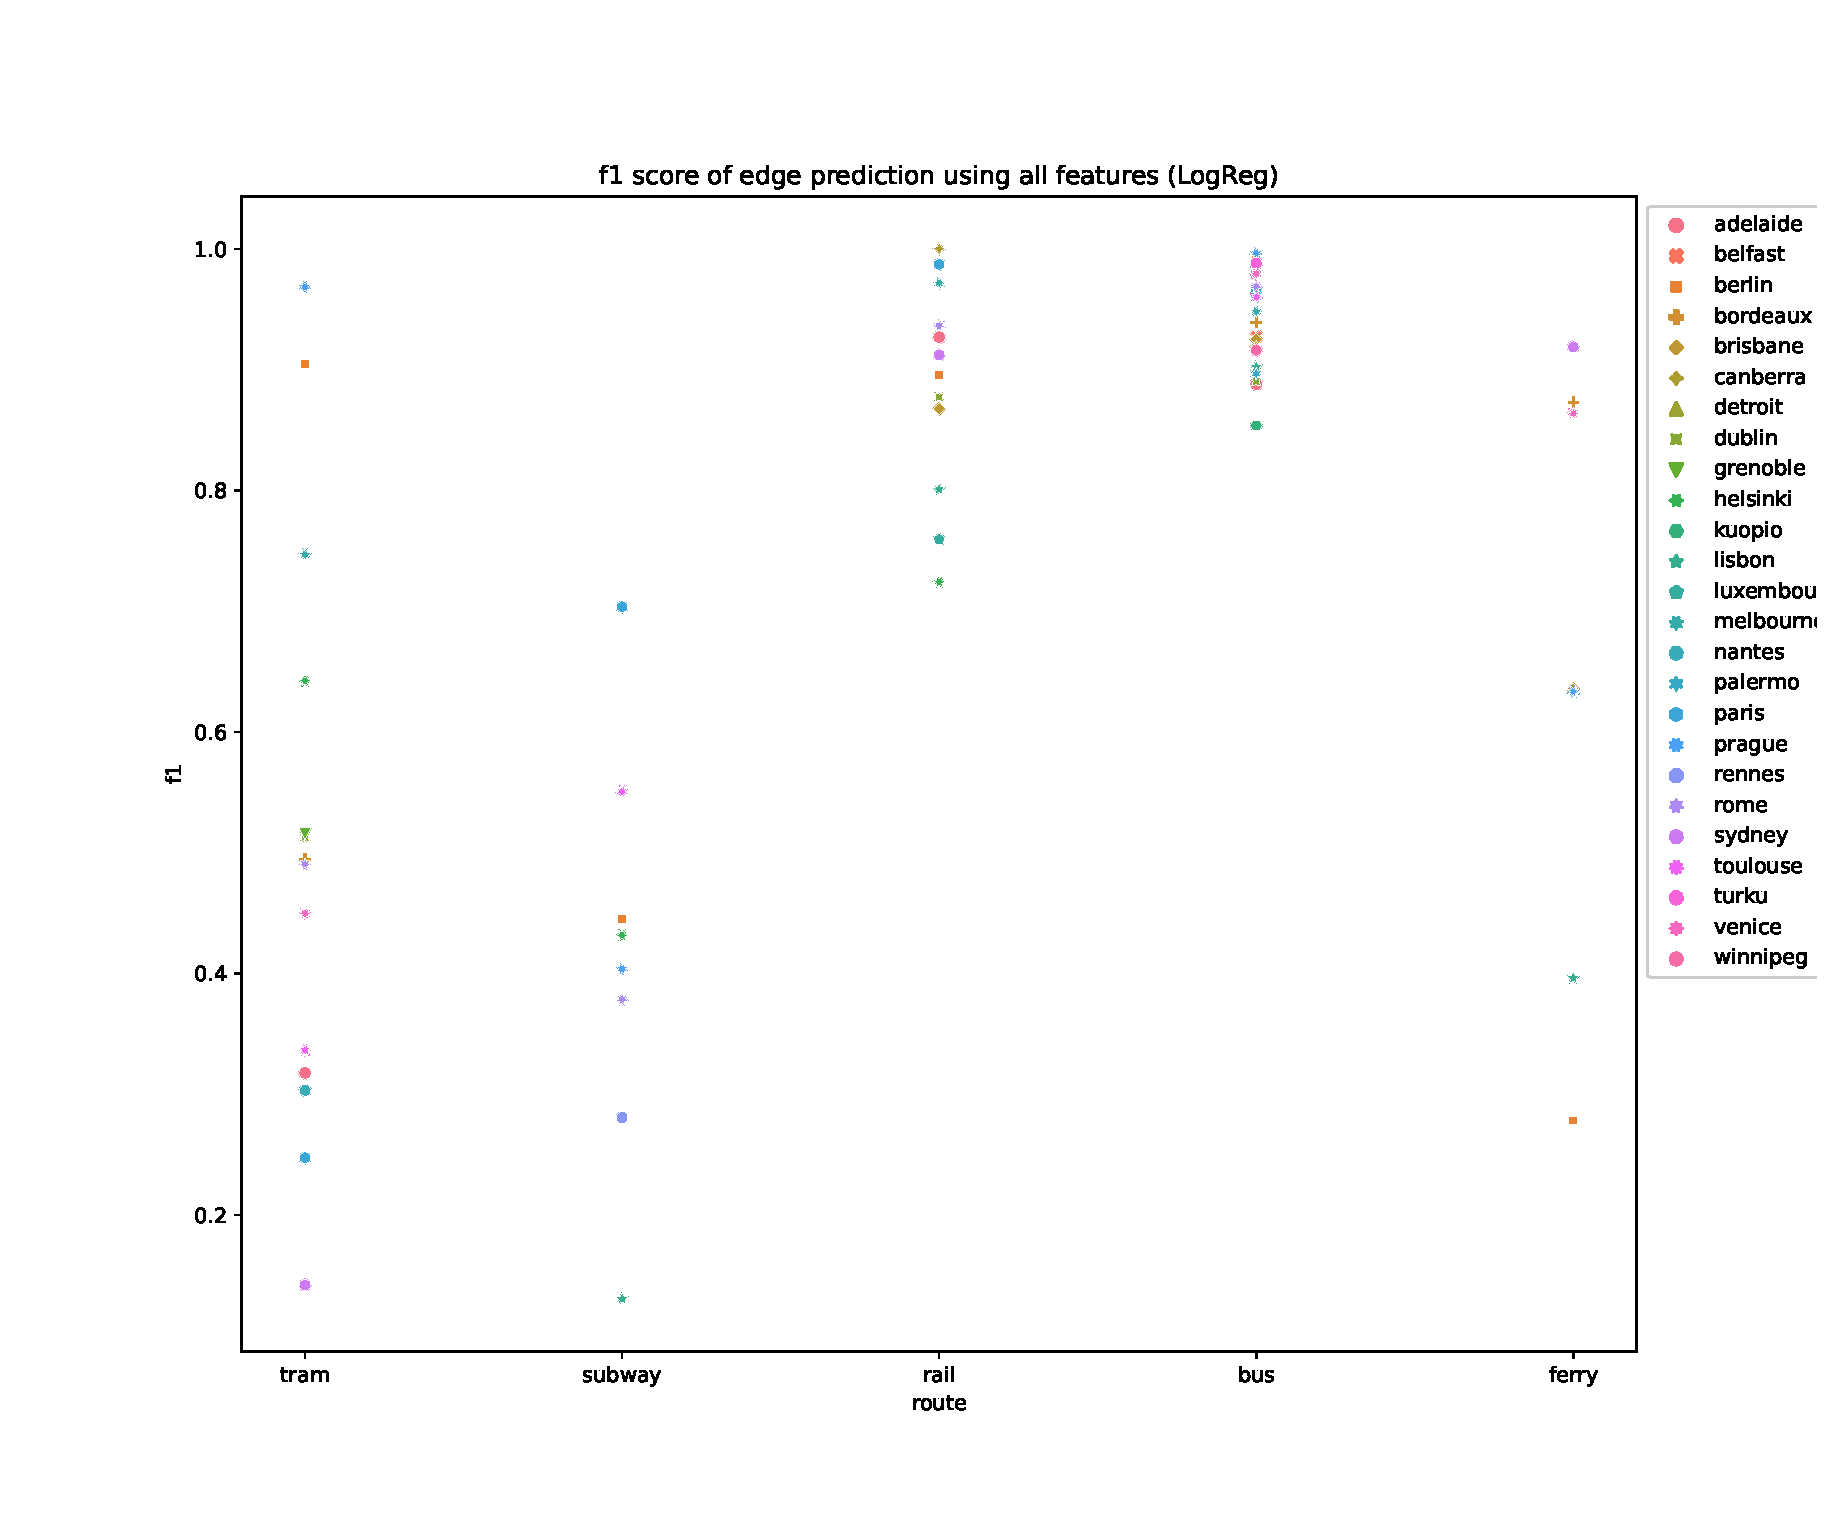
\includegraphics[width=\columnwidth]{images/edge-pred-all.eps}}
\caption{F1 score of edge prediction using both properties}
\label{edge-pred-all_fig}
\end{center}
\vskip -0.3in
\end{figure}

\textsc{Hand-crafted Features}

Figures \ref{edge-pred-node_fig}, \ref{edge-pred-common_fig} and \ref{edge-pred-all_fig} show the F1 scores of the models predicting edges for each mode in each city utilising the node features alone, the common features alone and both of them together, respectively. All the networks in the dataset are very sparse (see the section on density), making the chance that two nodes are connected very low. Given very small clustering coefficients and densities for most networks, the random chance of an edge existing between two nodes is also minuscule \cite{frossard_2023b}.

\textit{Bus}

Employing the node features, the model achieves an F1 score of more than 0.6 for all the cities and more than 0.9 for Melbourne, Canberra, Winnipeg and Lisbon. Similarly, using the shared properties between nodes, the F1 scores for all cities are higher than 0.99. Using all features together, the F1 scores start from 0.85 and go up. The average density of the bus networks is 0.001. In using common features, the regressor is learning to predict an edge if both of those values are zero. However, in denser networks and those networks that have more than one path to reach a node, the regressor is unable to perform well. In the same scenario, the F1 scores are inversely proportional to the densities i.e., the graphs with high density have low F1 scores, and those with low density have higher F1 scores. This is the only case where the results are related to a graph property.

\textit{Tram}

All 14 cities that have tram service have an F1 score greater than 0.5 and accuracies between 0.46 and 0.62 using the node properties as features. With common properties as features, the F1 scores go as low as 0.004 and as high as 0.988. The F1 score lies in the range of 0.14 and 0.96 when using both of them together. The average density of the tram networks is 0.03.

\textit{Rail}

In the 12 cities with Rail, with node properties, the F1 score is between 0.53 and 0.86. With common features, the F1 score is between 0.86 and 1.00. Using both of the features results in an F1 score between 0.72 and 1.00. In both cases, Canberra has a score of 1.0, but it only has three nodes with four edges. The average density of the rail networks is 0.08.

\textit{Subway}

Using node properties as features, the F1 score is in the range of 0.62 and 0.67 for the subway network, while the accuracy is in the 0.5 ballparks. The range changes to 0.035 and 0.98 with common properties and to 0.13 and 0.70 together. The average density of the subway networks is 0.05.

\textit{Ferry}

The F1 score for edge prediction in the ferry is between 0.56 and 0.85, while the accuracy is between 0.53 and 0.9 using the node properties. With the common features, this range changes to 0.13 to 0.95 and it becomes 0.27 to 0.91 with both of them together. The average density of the ferry networks is 0.21. 

In summary, for edge prediction on an individual mode of transport, the fraction of common incoming and outgoing neighbours are best suited for the bus and rail networks in all cities. Those features are also suitable for the ferry network in Bordeaux, Sydney and Venice, the Subway network in Paris and the Tram network in Berlin and Prague. Among the remaining cities for the ferry, Subway and trams, the node properties have performed better. Considering the very sparse networks with very low clustering coefficients, these prediction results show a large improvement.

\textsc{Node2Vec Features}

Figure \ref{edge-pred-n2v_fig} visualises the F1 scores for the task with varying number of features. The performance of the Node2Vec features for the bus networks drops significantly compared to the handcrafted features. The F1 scores for the bus network are in the ballpark of 0.67. For the tram network, the performance improves for many cities using the Node2Vec features. The node2vec features do not fare well for the rail network as well. The node2vec features for the subway network perform similarly to that of the node features considered earlier. Lastly, in ferry networks, there is a drop in performance for some cities, and others have the same performance as using the handcrafted features.

\begin{figure}[ht]
\vskip -0.1in
\begin{center}
\centerline{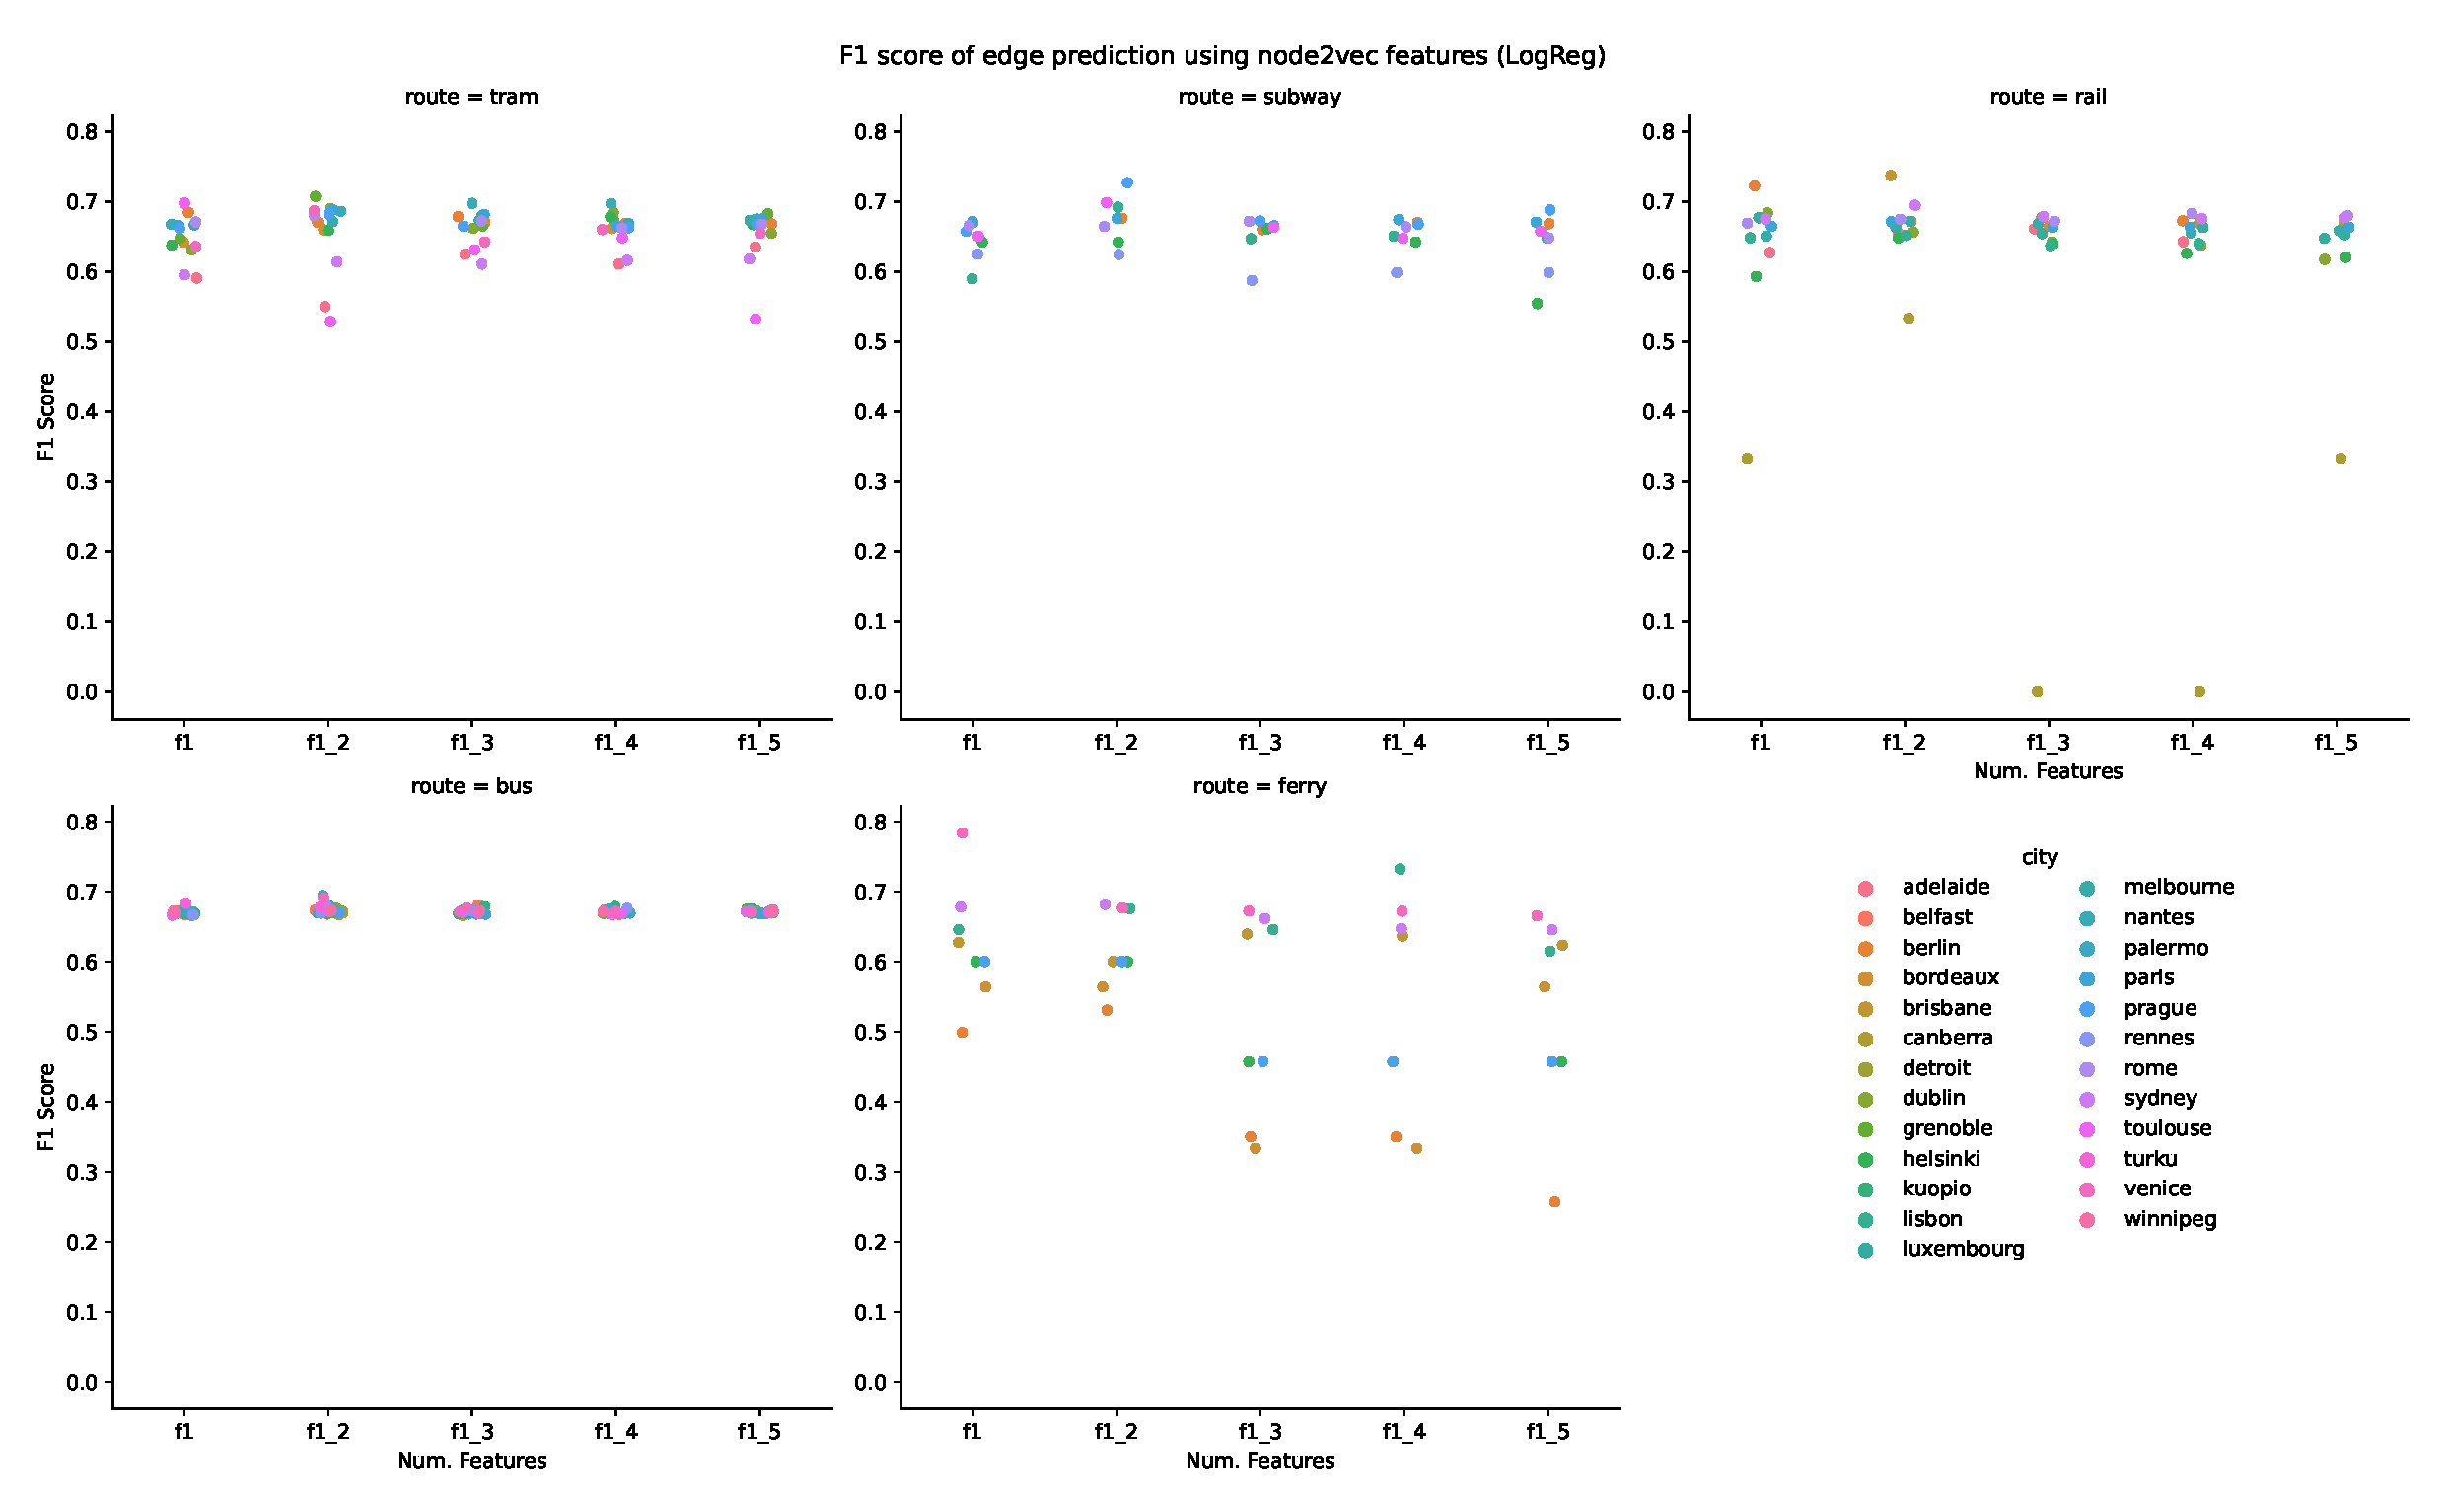
\includegraphics[width=\columnwidth]{images/edge-pred-node2vec.eps}}
\caption{F1 score of edge prediction using 1 to 5 Node2Vec features}
\label{edge-pred-n2v_fig}
\end{center}
\vskip -0.3in
\end{figure}

Overall, the Node2Vec features do not perform well for the bus, rail and ferry networks. The tram and subway networks perform better or are similar to the handcrafted features.

\textbf{Label Prediction}

\begin{figure}[ht]
\vskip -0.1in
\begin{center}
\centerline{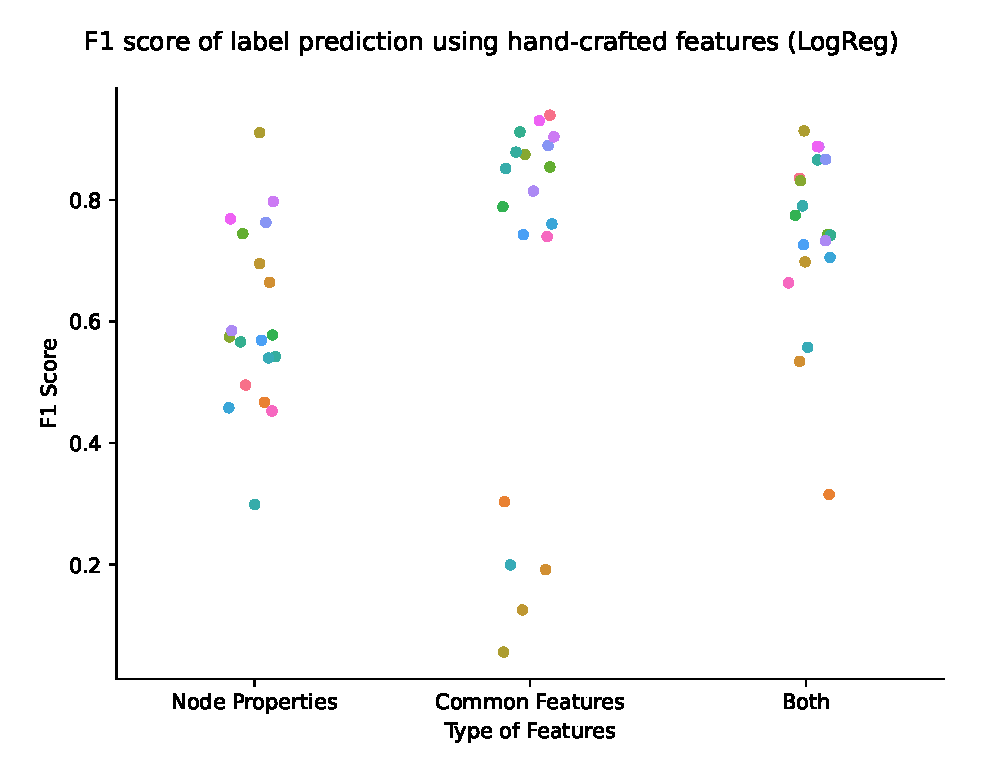
\includegraphics[width=\columnwidth]{images/label-pred-all_combined.eps}}
\caption{F1 score of label prediction using Hand Crafted features}
\label{label-pred-hc_fig}
\end{center}
\vskip -0.3in
\end{figure}

% \begin{figure}[ht]
% \vskip -0.1in
% \begin{center}
% \centerline{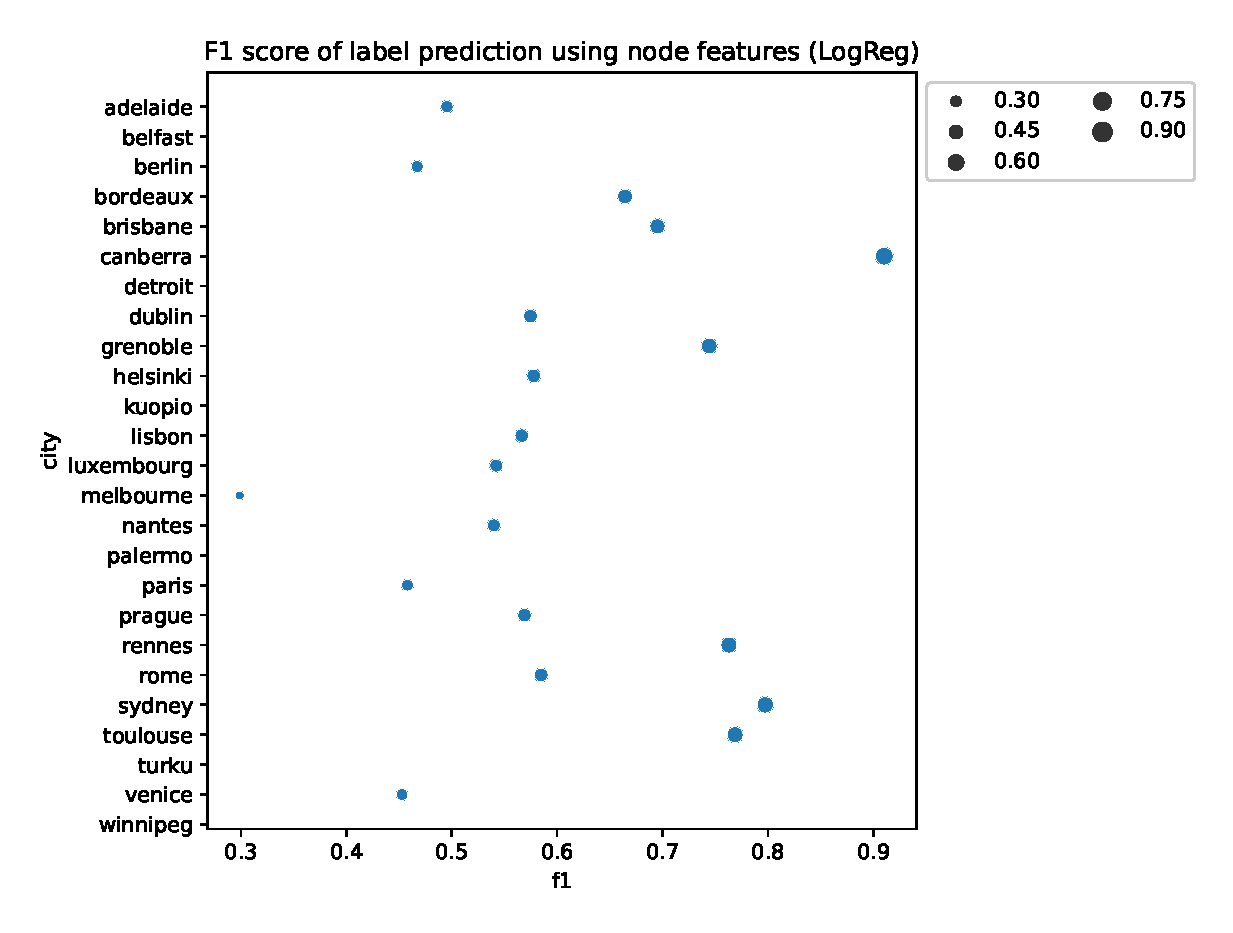
\includegraphics[width=\columnwidth]{images/label-pred-hco.eps}}
% \caption{F1 score of label prediction using node properties}
% \label{label-pred-node_fig}
% \end{center}
% \vskip -0.3in
% \end{figure}

% \begin{figure}[ht]
% \vskip -0.1in
% \begin{center}
% \centerline{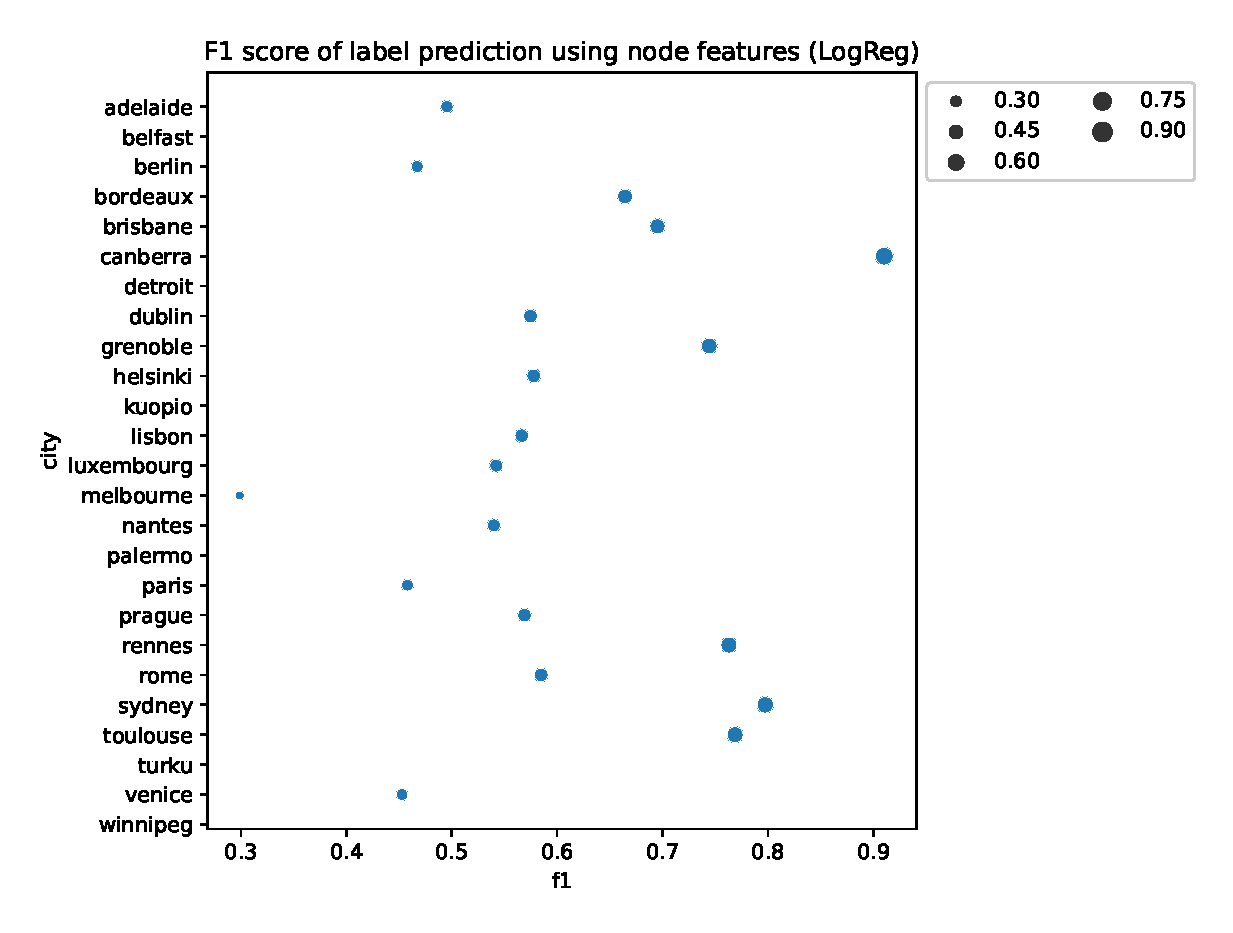
\includegraphics[width=\columnwidth]{images/label-pred-commono.eps}}
% \caption{F1 score of label prediction using common properties}
% \label{label-pred-common_fig}
% \end{center}
% \vskip -0.3in
% \end{figure}

% \begin{figure}[ht]
% \vskip -0.1in
% \begin{center}
% \centerline{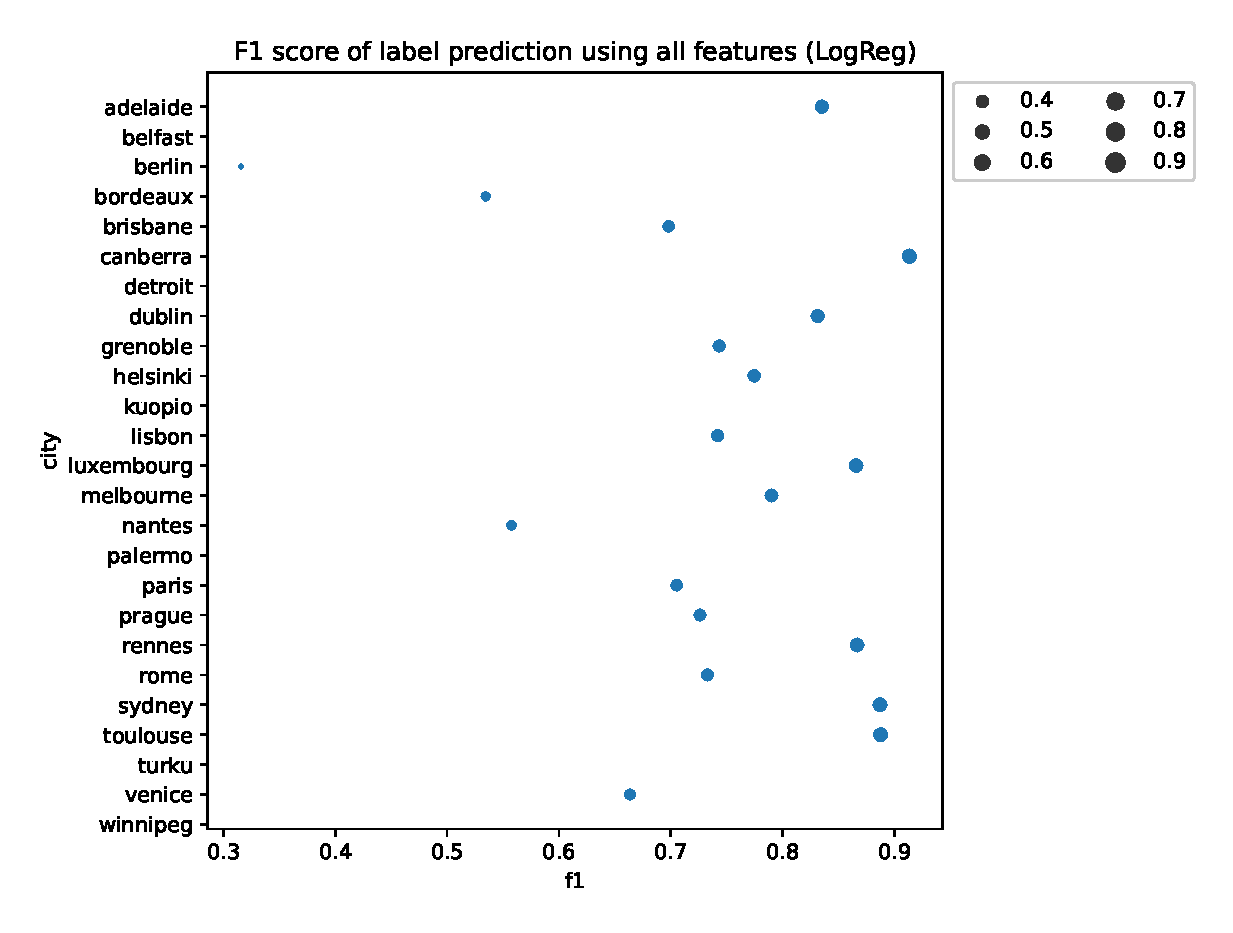
\includegraphics[width=\columnwidth]{images/label-pred-all.eps}}
% \caption{F1 score of label prediction using both properties}
% \label{label-pred-all_fig}
% \end{center}
% \vskip -0.3in
% \end{figure}

\textsc{Hand-crafted Features}

The label prediction task involves predicting the type of edge (represents the mode of transport) given that it already exists between two nodes. Thus, each city was trained on a model of its own, considering all the modes of transport it has. The number of samples was equal to the number of existing edges. However, the targets were an array with dimensions equal to the number of modes of transport in the city. Cities with only one mode of transport were excluded from the analysis. In the experiment with hand-crafted features, everything was similar to edge prediction except that the Katz centrality was removed from the node properties due to the complex MultiDiGraph structure.

Using only the node properties, the F1 scores (\cref{label-pred-hc_fig}) on the task were from 0.3 to 0.91. Since the bus network label is the most common, it was predicted often. Canberra achieves the highest score of 0.91. The city has two modes of transport (bus and rail). The bus network consists of 2727 nodes and 3209 edges, and the rail network has only 3 nodes and 4 edges. Such heavy imbalance gives rise to the high average F1 score. In contrast, Melbourne with three modes of transport - bus(13131 nodes, 18943 edges), tram (219 nodes, 563 edges), and rail (219 nodes and 563 edges) has the least score of 0.3. The model failed to capture the complexity of the problem with selected features.

On average many cities achieve better performance with common features than using the node properties (\cref{label-pred-hc_fig}). The F1 scores lie between 0.06 and 0.94. Adelaide, Lisbon, Sydney and Toulouse have an f1 score greater than 0.9. Looking at the confusion matrix reveals the same problem as earlier i.e., the weighted average of the score is high, but the individual label performances are not good. Canberra has the lowest f1 score of 0.06 and the confusion matrix shows that 97\% of the time, the rail label is predicted. A similar trend was seen in Berlin, Bordeaux and Brisbane which have F1 scores less than 0.4. Those cities with high scores predicted bus labels majorly, and those with least scores did not.

Lastly, when using both node and common features, the F1 score of all cities (\cref{label-pred-hc_fig}) except Berlin (the performance further drops) shows a significant improvement. The f1 score of Berlin is 0.32, which is the least followed by 0.52 for Bordeaux, 0.66 for Venice and more than 0.7 for the remaining. As expected, the ability (inability) to predict (not predict) the bus label influenced the average score. Nevertheless, using both features creates a hybrid model with better than random performance.

\textsc{Node2Vec Features}

\begin{figure}[ht]
\vskip -0.1in
\begin{center}
\centerline{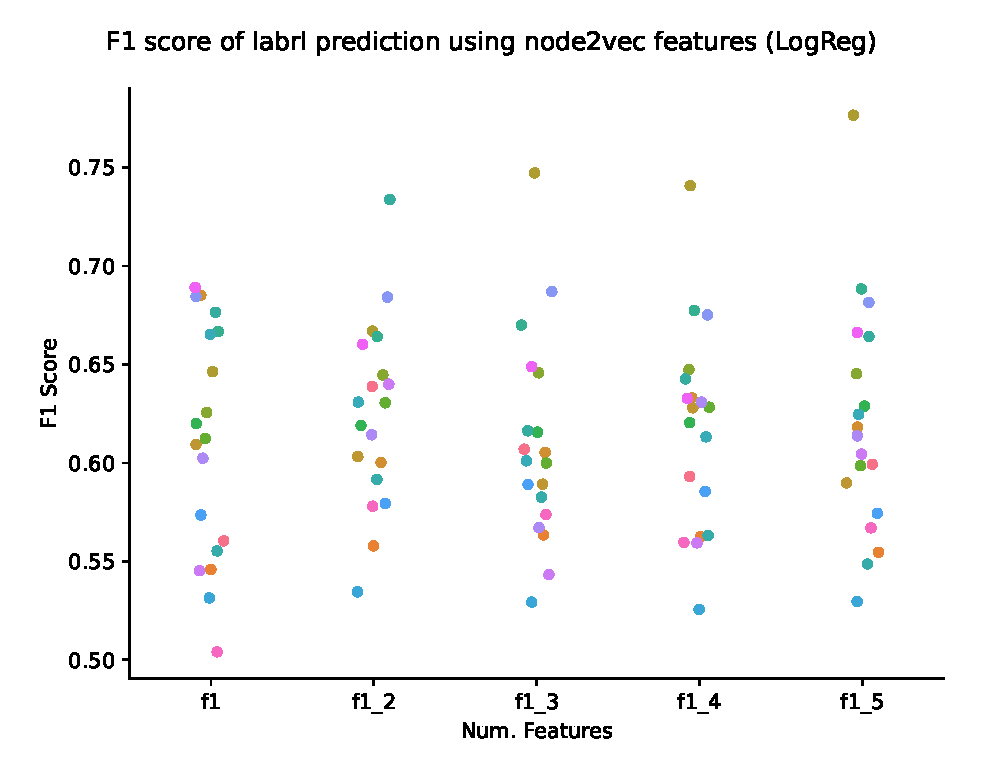
\includegraphics[width=\columnwidth]{images/label-pred-node2vec.eps}}
\caption{F1 score of label prediction using 1 to 5 Node2Vec features}
\label{label-pred-n2v_fig}
\end{center}
\vskip -0.3in
\end{figure}

For most of the cities, Node2Vec features do not even perform as well as using the common features (\cref{label-pred-n2v_fig}). However, for Berlin and Bordeaux Node2Vec improves compared to using node features, which was the best for them. For the city of Nantes, Node2Vec performs better than its best performer which uses the combined node and common features. 

Overall, the influence of the number of features on the performance of the model is not significant. Among the cities where Node2Vec performs better, Bordeaux and Nantes achieved the best performance with one feature, and Berlin with three.

\subsubsection{Graph Neural Networks}
The hand-crafted and Node2Vec features did not have consistency across all cities, and experiments were conducted using Graph Neural Networks (GNN) to see if the GNNs perform consistently. The experimental results revealed that this approach did not yield satisfactory performance for link and label prediction in transport networks. The probable reason could be that the complexity and inherent noise within transport networks may have posed challenges for the GNN to effectively capture and model the underlying dynamics. Additionally, the limited amount of labelled training data for transport networks might have impeded the network's ability to generalize and make accurate predictions. Especially the imbalance in the examples for different modes of transport.

It is worth noting that traditional approaches, such as hand-crafted and node2vec features, have demonstrated decent performance in similar prediction tasks. These methods rely on carefully engineered domain-specific features and embedding techniques that capture relevant characteristics of the transport network.

\section{Conclusion}
\label{conclusion}

This project analysed the transport system of 25 cities through network analysis. The initial investigation highlighted the pitfalls of lacking standardised nomenclature and aggregation rules of the stops. Other aspects revealed in the exploration are the unusually low density and clustering coefficient of the networks and their existence of hubs - properties that indicate that these are scale-free networks and not random. The Betweenness centrality spotlighted the network's critical stations that act as transit stops. Keeping track of these stations and their infrastructure will be crucial in maintaining the smooth operation of public transport in the city. The average degree of 2 confirms a general understanding of connectivity in the transport system - with the previous and next stop. The number of nodes with varied types of edges shows the connectedness of the network, and very few cities were well connected, but most were not. This information formed the basis for the tasks of edge prediction between the nodes and edge type(s) prediction.

The second part of the project involved edge and edge-label prediction using hand-crafted and Node2Vec features. Directed edges were predicted between two nodes, and separate experiments were conducted for each city and mode of transport. The hand-crafted features of in-degree centrality, out-degree centrality, betweenness centrality and Katz centrality were well suited, and the Node2Vec features were only comparable to tram and subway networks. The label prediction involved predicting all modes of transport that exist between the edges of the entire city. Label prediction also used the same hand-crafted features except for Katz centrality. In this second task, the hand-crafted features were well-suited for most of the cities. In both tasks, the number of Node2Vec features did not have any significant effect on the performance. The exploration of GNNs for link and label prediction in transport networks did not yield satisfactory results. Future research can focus on refining GNN architectures, incorporating additional contextual information, and exploring hybrid approaches to enhance their predictive capabilities. However, the success of traditional techniques could be attributed to their ability to incorporate domain-specific information effectively.

Although not severe, this study also has limitations. Firstly humans would mentally represent a stop as a single location irrespective of the number of platforms or on which side of the road is the boarding point. However, this was not always the case. In future experiments, merging geographically closely located nodes can become a part of the pre-processing step. The geographical dimensions of the city and other factors, like its population, area, and usage of public transport, were not part of the analysis. Reading the existing results with these factors collected at the same time as the data collection period will deepen the relevancy of the results. The limits on the computation power did not allow us to conduct large experiments. One such experiment can be measuring the performance of edge and label prediction models on a different city than those they were originally trained on. Although a cross-validation study was ongoing, its results are not reported here, a cross-validation will further strengthen the findings.


\bibliography{example_paper}
\bibliographystyle{icml2023}


%%%%%%%%%%%%%%%%%%%%%%%%%%%%%%%%%%%%%%%%%%%%%%%%%%%%%%%%%%%%%%%%%%%%%%%%%%%%%%%
%%%%%%%%%%%%%%%%%%%%%%%%%%%%%%%%%%%%%%%%%%%%%%%%%%%%%%%%%%%%%%%%%%%%%%%%%%%%%%%
% APPENDIX
%%%%%%%%%%%%%%%%%%%%%%%%%%%%%%%%%%%%%%%%%%%%%%%%%%%%%%%%%%%%%%%%%%%%%%%%%%%%%%%
%%%%%%%%%%%%%%%%%%%%%%%%%%%%%%%%%%%%%%%%%%%%%%%%%%%%%%%%%%%%%%%%%%%%%%%%%%%%%%%
% \newpage
% \appendix
% \onecolumn
% \section{You \emph{can} have an appendix here.}

% You can have as much text here as you want. The main body must be at most $8$ pages long.
% For the final version, one more page can be added.
% If you want, you can use an appendix like this one, even using the one-column format.
%%%%%%%%%%%%%%%%%%%%%%%%%%%%%%%%%%%%%%%%%%%%%%%%%%%%%%%%%%%%%%%%%%%%%%%%%%%%%%%
%%%%%%%%%%%%%%%%%%%%%%%%%%%%%%%%%%%%%%%%%%%%%%%%%%%%%%%%%%%%%%%%%%%%%%%%%%%%%%%


\end{document}


% This document was modified from the file originally made available by
% Pat Langley and Andrea Danyluk for ICML-2K. This version was created
% by Iain Murray in 2018, and modified by Alexandre Bouchard in
% 2019 and 2021 and by Csaba Szepesvari, Gang Niu and Sivan Sabato in 2022.
% Modified again in 2023 by Sivan Sabato and Jonathan Scarlett.
% Previous contributors include Dan Roy, Lise Getoor and Tobias
% Scheffer, which was slightly modified from the 2010 version by
% Thorsten Joachims & Johannes Fuernkranz, slightly modified from the
% 2009 version by Kiri Wagstaff and Sam Roweis's 2008 version, which is
% slightly modified from Prasad Tadepalli's 2007 version which is a
% lightly changed version of the previous year's version by Andrew
% Moore, which was in turn edited from those of Kristian Kersting and
% Codrina Lauth. Alex Smola contributed to the algorithmic style files.
